%----------------------------------------------------------------------
% File:				ANNmanual.tex
% By:				David Mount
% Last modified:	05/03/05
% Description:		User manual for ANN
%----------------------------------------------------------------------
% Copyright (c) 1997-2005 University of Maryland and Sunil Arya and
% David Mount.  All Rights Reserved.
% 
% This software and related documentation is part of the Approximate
% Nearest Neighbor Library (ANN).  This software is provided under
% the provisions of the Lesser GNU Public License (LGPL).  See the
% file ../ReadMe.txt for further information.
% 
% The University of Maryland (U.M.) and the authors make no
% representations about the suitability or fitness of this software for
% any purpose.  It is provided "as is" without express or implied
% warranty.
%----------------------------------------------------------------------
% History:
% Revision 0.1  03/04/98
%	Initial release
% Revision 1.0  04/01/05
%	Added comments to ann_sample code
%	Added clus_orth_flats distribution
%	Added clus_ellipsoids distribution
%	Changed name of standard kd-tree split rule from "standard" to "kd"
%	Added ANN logo to title page.
%	Added description of ANNcoordPrec.
%	Added description of thePoints, nPoints, and theDim.
%	Added description of load constructor.
%	Updated description of ANN_BD_CENTROID.
%	Changed dump file suffix in ann2fig from ".ann" to ".dmp".
% Revision 1.1  05/03/05
%	Added instructions for Microsoft compilations.
%	Added annkFRSearch information
%----------------------------------------------------------------------
\documentclass[11pt]{article}		% plain manuscript (11pt)
\usepackage{fullpage}
\usepackage{amsmath}				% AMS math
\usepackage{amssymb}				% special AMS math symbols
\usepackage{graphicx}
\usepackage{url}
%-----------------------------------------------------------------------
%
%	Math shortcuts - floor, ceiling, ...
%
%-----------------------------------------------------------------------
\newcommand\floor[1]{\left\lfloor #1\right\rfloor}
\newcommand\ceil[1]{\left\lceil #1\right\rceil}
\newcommand\ang[1]{\langle #1\rangle}
%-----------------------------------------------------------------------
%  Tighter list environments
%-----------------------------------------------------------------------
\newenvironment{enumerate*}%            % Tighter enumerated list
  {\begin{enumerate}%
    \setlength{\itemsep}{-0.5ex}%
    \setlength{\parsep}{0pt}}%
  {\end{enumerate}}
\newenvironment{itemize*}%              % Tighter itemized list
  {\begin{itemize}%
    \setlength{\itemsep}{-0.5ex}%
    \setlength{\parsep}{0pt}}%
  {\end{itemize}}
\newenvironment{description*}%          % Tighter decsription list
  {\begin{description}%
    \setlength{\itemsep}{-0.5ex}%
    \setlength{\parsep}{0pt}}%
  {\end{description}}
%-----------------------------------------------------------------------
%
%	Typing shortcuts
%
%-----------------------------------------------------------------------
\newcommand{\ANN}[0]{\textsf{ANN}}
\newcommand{\ANNversion}[0]{1.1}
\newcommand{\ANNyear}[0]{2010}
\newcommand{\anntest}[0]{\textsf{ann\_test}}
\newcommand{\annsample}[0]{\textsf{ann\_sample}}
\newcommand{\annfig}[0]{\textsf{ann2fig}}
\newcommand{\dist}[0]{{\rm dist}}
\newcommand{\ROOT}[0]{\textit{root}}
\newcommand{\POW}[0]{\textit{pow}}
\newcommand{\DIFF}[0]{\ominus}
\newcommand{\SUM}[0]{\oplus}
\newcommand{\STRING}[0]{$\ang{\textit{string}\/}$}
\newcommand{\FILE}[0]{$\ang{\textit{file}\/}$}
\newcommand{\INT}[0]{$\ang{\textit{int}\/}$}
\newcommand{\FLOAT}[0]{$\ang{\textit{float}\/}$}
\newcommand{\RE}{\mathbb{R}}			% real space
\newcommand{\BSL}{\hbox{$\backslash$}}

\begin{document}
\bibliographystyle{alpha}
\pagenumbering{roman}
\setcounter{page}{0}

\title{ANN Programming Manual}

\author{David M. Mount\thanks{Email: \textsf{mount@cs.umd.edu}.
		The support of the National Science Foundation under
		grants CCR--9712379 and CCR-0098151 is gratefully
		acknowledged.}\\
	Department of Computer Science and \\
	Institute for Advanced Computer Studies \\
	University of Maryland, College Park, Maryland.
	}

\date{{\ANN}, Version {\ANNversion}\\
	Copyright, {\ANNyear}
	David M. Mount \\
	~ \\
	\centerline{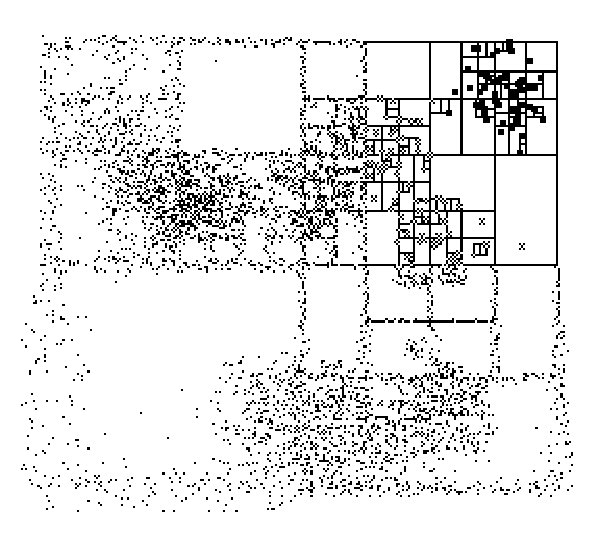
\includegraphics[height=2.0in]{Figs/annlogo.eps}}
    }

\maketitle
\thispagestyle{empty}

\newpage
\tableofcontents
\newpage
\pagenumbering{arabic}
\setcounter{page}{1}

%----------------------------------------------------------------------
\section{Introduction}
%----------------------------------------------------------------------

%----------------------------------------------------------------------
\subsection{What is {\ANN}?}
%----------------------------------------------------------------------

{\ANN} is a library written in the C++ programming language to support
both exact and approximate nearest neighbor searching in spaces of
various dimensions.  It was implemented by David M. Mount of the
University of Maryland and Sunil Arya of the Hong Kong University of
Science and Technology.  {\ANN} (pronounced like the name ``Ann'')
stands for the \emph{Approximate Nearest Neighbor} library.  {\ANN} is
also a testbed containing programs and procedures for generating data
sets, collecting and analyzing statistics on the performance of nearest
neighbor algorithms and data structures, and visualizing the geometric
structure of these data structures.

In the \emph{nearest neighbor problem} a set $P$ of data points in
$d$-dimensional space is given.  These points are preprocessed into a
data structure, so that given any query point $q$, the nearest (or
generally $k$ nearest) points of $P$ to $q$ can be reported efficiently.
{\ANN} is designed for data sets that are small enough that the search
structure can be stored in main memory (in contrast to approaches from
databases that assume that the data resides in secondary storage).
Points are assumed to be represented as coordinate vectors of reals (or
integers). The distance between two points can be defined in many ways.
{\ANN} assumes that distances are measured using any class of distance
functions called \emph{Minkowski metrics}.  These include the well known
Euclidean distance, Manhattan distance, and max distance.

Answering nearest neighbor queries efficiently, especially in higher
dimensions, seems to be very difficult problem.  It is always possible
to answer any query by a simple brute-force process of computing the
distances between the query point and each of the data points, but this
may be too slow for many applications that require that a large number
of queries be answered on the same data set.  Instead the approach is to
preprocess a set of data points into a data structure from which nearest
neighbor queries are then answered.  There are a number of data
structures that have been proposed for solving this problem.  See, for
example, \cite{AMN98,Ben90,Cla97,Kle97,PrS85,Spr91}, for more
information on this problem.

One difficulty with exact nearest neighbor searching is that for
virtually all methods other than brute-force search, the running time or
space grows exponentially as a function of dimension.  Consequently
these methods are often not significantly better than brute-force
search, except in fairly small dimensions.  However, it has been shown
by Arya and Mount \cite{ArM93} and Arya, et al.~\cite{AMN98} that if the
user is willing to tolerate a small amount of error in the search
(returning a point that may not be the nearest neighbor, but is not
significantly further away from the query point than the true nearest
neighbor) then it is possible to achieve significant improvements in
running time. {\ANN} is a system for answering nearest neighbor queries
both \emph{exactly} and \emph{approximately}.

This manual describes how to download and install {\ANN}, how to use the
library, how to change its configuration for different distance
functions and data representations, and finally how to use its utility
programs for testing and visualizing the data structure.

%----------------------------------------------------------------------
\subsection{Downloading and Using {\ANN}}
%----------------------------------------------------------------------

The current version of {\ANN} is version {\ANNversion}.  The {\ANN} source
code and documentation is available from the {\ANN} web page:
\begin{center}
    \url{http://www.cs.umd.edu/~mount/ANN}
\end{center}

The unbundled software consists of the following major files and
directories.
%
\begin{description*}
\item[\hbox{\sf ReadMe.txt:}] General description of the library.
\item[\hbox{\sf Copyright.txt:}] Copyright information.
\item[\hbox{\sf License.txt:}] Conditions of use for the library.
\item[\hbox{\sf include:}] Include files for compiling programs that use
	the library.
\item[\hbox{\sf src:}] The source files for the library.
\item[\hbox{\sf sample:}] A small sample program, which illustrates
	how to input a point set, build a search structure for the set, and
	answer nearest neighbor queries. (See Section~\ref{annsample.sec}.)
\item[\hbox{\sf test:}] A program that provides a simple script
	input for building search trees and comparing their performance on
	point sets that are either read from an input file or generated
	according to some probability distribution. (See
	Section~\ref{anntest.sec}.)
\item[\hbox{\sf ann2fig:}] A program that generates a visual
	representation (in fig format) of the tree's spatial decomposition.
	(See Section~\ref{ann2fig.sec}.)
\item[\hbox{\sf lib:}] Where the compiled library is stored.
\item[\hbox{\sf bin:}] Where the compiled executables are stored.
\item[\hbox{\sf doc:}] This documentation.
\item[\hbox{\sf MS\_Win32:}] Solution and project files for compilation
	under Microsoft Visual Studio~.NET.
\end{description*}

%----------------------------------------------------------------------
\subsection{Compiling {\ANN}}
%----------------------------------------------------------------------

{\ANN} requires an ANSI standard C++ compiler.  It has been compiled
successfully on Unix and Linux systems including Sun Workstations
running SunOS 5.X (Solaris), Linux Red Hat 2.X, and on DEC Alphas
running Digital Unix v4.X, on SGIs running IRIX 6.X.  Makefiles for all
these systems.  It has also been compiled under Microsoft Windows XP
(under Visual Studio~.NET).

\subsubsection{Compiling on Unix/Linux Systems}

After downloading the sources, change to the {\ANN} root directory (from
which directories such as \textsf{bin}, \textsf{doc}, and
\textsf{include} branch off) and enter the command ``\textsf{make}''.  This
will provide a list of platforms and options under which to compile
{\ANN}.  If you do not see your particular configuration on this list,
then you might try modifying the file \textsf{Make-config} for your
particular system.  The authors welcome any additions to the list of
supported platforms.

There are some additional compilation options that can be enabled or
disabled.  These are described in Section~\ref{compileopt.sec}.  To
recompile the library, enter the command ``\textsf{make realclean}'' to
delete the library and utility programs, and then reenter the make
command for compilation.

\subsubsection{Compiling on Microsoft Windows Systems}

To compile under Visual C++ running within Microsoft Visual Studio~.NET,
go to the directory \textsf{MS\_Win32}.  Open the solution file
\textsf{Ann.sln}, select the ``Release'' configuration, and select
``Build $\rightarrow$ Build Solution.''  After compilation, the file
\textsf{ANN.lib} is stored in the directory
\textsf{MS\_Win32{\BSL}dll{\BSL}Release}.  The file \textsf{ANN.dll}
file and executables of the utility programs are stored in the directory
\textsf{bin} (relative to the {\ANN} root directory).  These two files,
along with the files in the directory \textsf{include/ANN} are needed
for compiling applications that use {\ANN}.

\subsubsection{Precompiled Files for Microsoft Windows}

For Microsoft Windows users that do not need to modify the software, a
bundle containing all the files you need to use {\ANN} has been
provided.  This contains the include files in \textsf{include/ANN} along
with \textsf{ANN.lib} and \textsf{ANN.dll}.  It can be downloaded
directly from \url{http://www.cs.umd.edu/~mount/ANN}.  In order to use
these with an application it is necessary to copy each of these files to
appropriate directories for the compiler and linker to locate them, and
then to set the appropriate compiler, linker, and path settings so the
system can locate all these files. You should consult your local system
documentation for this information. An example of how to do this for the
sample program is given in Section~\ref{compilesample.sec}.

%----------------------------------------------------------------------
\subsection{Compiling Applications that Use the Library}
%----------------------------------------------------------------------

In order to use {\ANN} in a C++ program, the program must include the
header file for {\ANN}, which contains the declarations for the {\ANN}
objects and procedures.  This is done with the following statement in
the C++ source code.

{\small \begin{verbatim}
    #include <ANN/ANN.h>
\end{verbatim} }

This assumes that the {\ANN} include directory is already on the
compiler's search path for include files.  On most Unix/Linux-based C++
compilers, this is done by setting the ``-I'' (capital letter ``i'')
option on the compilation command line to point to the include directory
in the {\ANN} base directory.

Then the program is linked with the {\ANN} library.  On Unix/Linux-based
systems this is done with the ``\textsf{-l}'' (lower-case letter
``$\ell$'') option, assuming that the library search path has been set
to include the {\ANN} library directory.  The library search path can be
set with the ``\textsf{-L}'' option.   For example, on my Unix system,
the following command line could be used to compile the program
\textsf{my\_program.cpp} using the {\ANN} library and the GNU C++
compiler.  Let \textsf{ann} denote the path to root {\ANN} directory.

{\small \begin{verbatim}
    g++ my_program.cpp -Iann/include -Lann/lib -lANN
\end{verbatim} }

Some additional information on compiling applications that use {\ANN} on
Microsoft Windows systems can be found in
Section~\ref{compilesample.sec}.

%----------------------------------------------------------------------
\newpage
\section{The {\ANN} Library}\label{annlib.sec}
%----------------------------------------------------------------------

{\ANN} is a library of C++ objects and procedures that supports
approximate nearest neighbor searching.  In \emph{nearest neighbor
searching}, we are given a set of data points $S$ in real
$d$-dimensional space, $\RE^d$, and are to build a data structure such
that, given any query point $q \in \RE^d$, the nearest data point to $q$
can be found efficiently.  In general, we are given $k \ge 1$, and are
asked to return the $k$-nearest neighbors to $q$ in $S$.

In \emph{approximate nearest neighbor searching}, an error bound
$\epsilon \ge 0$ is also given.  The search algorithm returns $k$
distinct points of $S$, such that for $1 \le i \le k$, the ratio between
the distance to the $i$th reported point and the true $i$th nearest
neighbor is at most $1+\epsilon$.

\ANN's features include the following.
\begin{itemize}
\item	It supports $k$-nearest neighbor searching, by specifying $k$
	with the query.
\item	It supports both exact and approximate nearest neighbor searching,
	by specifying an approximation factor $\epsilon \ge 0$ with
	the query.
\item	It supports any Minkowski distance metric, including the $L_1$
	(Manhattan), $L_2$ (Euclidean), and $L_{\infty}$ (Max) metrics.
\item	Preprocessing time and space are both linear in the number of
	points $n$ and the dimension $d$, and are independent of $\epsilon$.
	Thus the data structure requires storage that is only moderately
	larger than the underlying data set.
\end{itemize}

{\ANN} was written as a testbed for a class of nearest neighbor
searching algorithms, particularly those based on orthogonal
decompositions of space.  These include kd-trees \cite{Ben90,FBF77}, and
box-decomposition trees \cite{AMN98}.  These will be described in
Section~\ref{structs.sec}.  The library supports a number of different
methods for building these search structures.  It also supports two
methods for searching these structures: standard tree-ordered search
\cite{ArM93b} and priority search \cite{AMN98}.  These will be described
in Section~\ref{search.sec}.

In addition to the library there are two programs provided for testing
and evaluating the performance of various search methods.  The first,
called {\anntest}, provides a primitive script language that allows the
user to generate data sets and query sets, either by reading from a file
or randomly through the use of a number of built-in point distributions.
Any of a number of nearest neighbor search structures can be built, and
queries can be run through this structure.  This program outputs a
number of performance statistics, including the average execution time,
number of nodes visited in the data structure, and the average error
made in the case of approximate nearest neighbors.  An operation is
provided to have the data structure dumped to a file and to load the
data structure from a dumped file.

The second program, called {\annfig}, takes the dumped data structure
and generates an illustration of the data structure, which is output to
a file in a simple graphics format.  When the dimension is higher than
two, this program can output any planar 2-dimensional ``slice'' of the
data structure.  An example is shown in Figure~\ref{ann.fig}.  The
output of {\annfig} is the same format used by the Unix program xfig.
Through the Unix program \textsf{fig2dev}, it is possible to convert
this format to a number of other picture formats, including encapsulated
postscript.

\begin{figure}[htbp]
  \centerline{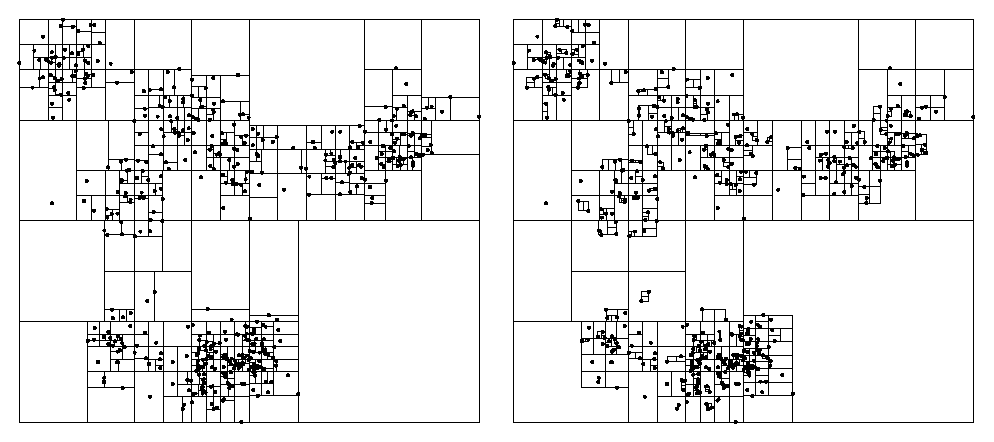
\includegraphics[height=2.0in]{Figs/ann.eps}}
  \caption{Sample output of {\annfig} for a kd-tree and a
  box-decomposition tree.}
  \label{ann.fig}
\end{figure}

%----------------------------------------------------------------------
\subsection{Using {\ANN}}\label{using.sec}
%----------------------------------------------------------------------

This section discusses how to use {\ANN} for answering nearest neighbors
in its default configuration, namely computing the nearest neighbor
using Euclidean distance for points whose coordinates are of type
\textsf{double}.  Later in Section~\ref{custom.sec} we discuss how to
customize {\ANN} for different coordinate types and different norms.

\subsubsection{Coordinates, Points, Distances, and Indices}\label{point.sec}

Each point in $d$-dimensional space is assumed to be expressed as a
$d$-vector of coordinates
\[
	p = (p_0, p_1, \ldots, p_{d-1}).
\]
(Indices start from 0, as is C++'s convention.)  A coordinate is of type
\textsf{ANNcoord}.  By default, \textsf{ANNcoord} is defined to be of
type \textsf{double}, but it is possible to modify the {\ANN} include
files to change this and other {\ANN} types, as described in
Section~\ref{point2.sec}.

{\ANN} defines the distance between two points to be their Euclidean
distance, that is
\[
    \dist(p,q) = \left(\sum_{0 \le i < d} (p_i-q_i)^2 \right)^{1/2}.
\]
(Section~\ref{norm.sec} explains how to modify {\ANN} for other
Minkowski norms.)  For the purposes of comparing distances, it is not
necessary to compute the final square root in the above expression.
{\ANN} actually computes \emph{squared distances} rather than true
Euclidean distances.  A squared distance is defined to be of type
\textsf{ANNdist}.  It is defined to be \textsf{double} by default (but
can be changed).  By using squared distances rather than true Euclidean
distances, {\ANN} not only saves on the time of computing square roots,
but has the advantage that integer types can be used instead to
accurately represent distances when integer type coordinates are used.
(It worth emphasizing that, even though {\ANN} represents distances
internally as squared distances, when it computes $\epsilon$-approximate
nearest neighbors, the approximation is relative to the true, not
squared, distance.)

The most basic object manipulated by {\ANN} is a \emph{point}, which is
defined in C++ to be a dimensionless array of coordinates, or more
simply a pointer to a coordinate.%
%
\footnote{It is natural to wonder why {\ANN} does not define a special
point class, which might store additional information about points.
This would then necessitate that the library be templated about the
point type.  Since compiler support for templating was rather weak in
the mid-90's when {\ANN} was first implemented designed, it was decided
instead to decouple the user's point object from the {\ANN} point type.
In this way we allow the user to define a point object in any way
desired.  The user then interfaces with {\ANN} by simply providing a
pointer to the point's coordinates.  In many cases, this may just be a
field in the user's own point class.}
%
Thus we define \textsf{ANNpoint} to be
{\small \begin{verbatim}
    typedef ANNcoord* ANNpoint;         // a point
\end{verbatim} }
It is the user's responsibility to allocate and deallocate storage
for points.  Each point must have at least as many components allocated
as the dimension of the space.  Any extra components are ignored.

Since {\ANN} operates on arrays of points and distances, we also define
dimensionless arrays of these two objects:
%
{\small \begin{verbatim}
    typedef ANNpoint* ANNpointArray;    // an array of points
    typedef ANNdist*  ANNdistArray;     // an array of squared distances
\end{verbatim} }

We will see later that a set of data points is presented to {\ANN} as an
\textsf{ANNpointArray}.  {\ANN} returns the results of a nearest
neighbor query as an integer index into this array.  To make it clear
when we are doing so, {\ANN} defines the type \textsf{ANNidx} to be a
psuedonym for \textsf{int}.  The result of a $k$-nearest neighbor query
is returned as a pointer to an array of indices, which is of type
\textsf{ANNidxArray}, defined as follows.
%
{\small \begin{verbatim}
    typedef ANNidx*   ANNidxArray;      // an array of point indices
\end{verbatim} }

Finally, {\ANN} provides a boolean type called \textsf{ANNbool}.
(Although ANSI C++ provides a type \textsf{bool}, this is not supported
in some of the older compilers.)  Its values are \textsf{ANNfalse} and
\textsf{ANNtrue}.

\subsubsection{Nearest Neighbor Search Structure}\label{struct.sec}

The principal structure that {\ANN} uses for performing nearest neighbor
searches is called an \textsf{ANNpointSet}.  This is an abstract object
which supports two search operations, \textsf{annkSearch()}, which
computes the approximate $k$ nearest neighbors of a query point, and
\textsf{annKFRSearch()}, which performs a combination of a fixed-radius
approximate $k$ nearest neighbor search and a range search (see the
description below).

{\ANN} provides three concrete instantiations of an
\textsf{ANNpointSet}: \textsf{ANNbruteForce}, \textsf{ANNkd\_tree}, and
\textsf{ANNbd\_tree}.  The first of these stores the points as an array,
and implements a simple brute-force search for nearest neighbors.  It is
provided primarily for the use of the implementors to validate the
correctness of the more sophisticated search structures, and should not
be used for actual nearest neighbor queries.  Among the other two, we
will first introduce only the more basic one, the \textsf{ANNkd\_tree},
and leave the \textsf{ANNbd\_tree} to be discussed in
Section~\ref{struct2.sec}.  The \textsf{ANNkd\_tree} supports the
following operations.

\begin{description}
\item[Constructor:] This builds a kd-tree from a set of $n$ data points
	in dimension $d$, stored in a point array $pa$.  The procedure
	allocates the necessary storage for the data structure.  It is
	assumed that there is at least one data point ($n \ge 1$) and
	that the dimension is strictly positive ($d \ge 1$).  Warning:
	This procedure does virtually no error checking, and if these
	assumptions are violated or if storage cannot be allocated, then
	the most likely result will be that the program aborts.
	
	A (simplified) prototype is given below.  (See
	Section~\ref{struct2.sec} for more complete information.)  The order
	in which the points appear in the points array is significant,
	because nearest neighbors are returned by their index in this array.
	Following C++ conventions, the items are indexed from 0 to $n-1$.
	{\small \begin{verbatim}
	    ANNkd_tree::ANNkd_tree(
	        ANNpointArray   pa,             // data point array
	        int             n,              // number of points
	        int             d);             // dimension
	\end{verbatim} }

	To conserve space, the tree does not actually store the data
	points, but rather stores pointers to the array $pa$.  For this
	reason the contents of $pa$ should be unchanged throughout the
	lifetime of the data structure.

\item[$k$-Nearest Neighbor Search:] This member function is given a
	query point $q$, a nonnegative integer $k$, an array of point
	indices, \textit{nn\_idx}, and an array of distances,
	\textit{dists}.  Both arrays are assumed to contain at least $k$
	elements.  The procedure computes the $k$ nearest neighbors to $q$
	in the point set, and stores the indices of the nearest neighbors
	(relative to the point array \textit{pa} given in the constructor).
	The nearest neighbor is stored in $\textit{nn\_idx}[0]$, the second
	nearest in $\textit{nn\_idx}[1]$, and so on.  The \emph{squared}
	distances to the corresponding points are stored in the array
	\textit{dists}.

	Optionally, a real value $\epsilon \ge 0$ may be supplied.  If so,
	then the $i$th nearest neighbor is a $(1+\epsilon)$ approximation
	to the true $i$th nearest neighbor.  That is, the true (not squared)
	distance to this point may exceed the true distance to the real
	$i$th nearest neighbor of $q$ by a factor of $(1+\epsilon)$.  If
	$\epsilon$ is omitted then nearest neighbors are computed exactly.

	{\ANN} supports two different methods for searching the kd-tree.
	Here we present the simpler one, which is the more efficient for
	small values of $\epsilon$.  Another searching algorithm, called
	priority search, is presented later in Section~\ref{prsearch.sec}.

	{\small \begin{verbatim}
	    virtual void ANNkd_tree::annkSearch(
	        ANNpoint        q,            // query point
	        int             k,            // number of near neighbors to find
	        ANNidxArray     nn_idx,       // nearest neighbor array (modified)
	        ANNdistArray    dists,        // dist to near neighbors (modified)
	        double          eps=0.0);     // error bound
	\end{verbatim} }

\item[Fixed-radius $k$-Nearest Neighbor Search:] This member function is
	a modification of the above procedure, which searches for up to $k$
	nearest neighbors, but confines the search to a fixed radius bound.
	It is given a query point $q$, a (squared) radius bound
	\textit{sqRad}, a nonnegative integer $k$.  Optionally, it is given
	an array of point indices, \textit{nn\_idx}, an array of distances,
	\textit{dists}.  If provided, both arrays are assumed to contain at
	least $k$ elements.

	This procedure performs two different types of search.  First, if
	$k$ is positive and the two arrays \textit{nn\_idx} and
	\textit{dists} are provided, then among the points whose squared
	distance from $q$ is at most \textit{sqRad}, it finds the $k$
	closest of these to $q$.  If the number of points within the squared
	radius bound is some value $k'< k$, then only the first $k'$ entries
	of these arrays have meaningful entries.  The other entries of
	\textit{nn\_idx} contain the special value \textit{ANN\_NULL\_IDX}
	and the other entries of \textit{dists} contain the special value
	\textit{ANN\_DIST\_INF} (which are defined in \textsf{ANN.h}).

	This is called a fixed-radius search, because it ignores all the
	points that lie outside of the radius bound.  It is not however, a
	true fixed-radius search, because it computes only the closest $k$
	points that lie within the radius bound.  Thus, if the value of $k$
	is less than the total number of points $k'$ in the radius bound,
	the farthest $k'-k$ points within the radius will not be reported.
	(This limitation is because {\ANN} allocates all its arrays
	statically.)
	
	It is easy, however, to determine whether any points were missed.
	The procedure returns a count of the total number of points that lie
	within the radius bound.  (This feature is always enabled, even if
	$k = 0$.) In order to produce a true fixed-radius search, first set
	$k=0$ and run the procedure in order to obtain the number $k'$ of
	points that lie within the radius bound.  Then, allocate index and
	distance arrays of size $k'$ each, and repeat the fixed-radius
	search by setting $k=k'$ and passing in these two arrays.

	Optionally, a real value $\epsilon \ge 0$ may be supplied.  If so,
	the squared radius bound is treated as an approximate quantity in
	the following sense.  Assuming that we are using Euclidean
	distances, let $r = \sqrt{\textit{sqRad}}$ be the true radius bound.
	Every data point whose distance from $q$ is less than
	$r/(1+\epsilon)$ will be considered, and any point whose distance
	from $q$ is greater than $r$ will not be considered.  The remaining
	points either may or may not be considered (at the discretion of the
	search algorithm). Among the points that are considered, the $i$th
	elements of \textit{nn\_idx} and \textit{dists} contain the $i$th
	closest point to $q$, and the procedure returns a count of all the
	points under consideration.

	Here is the prototype of the fixed-radius search procedure.

	{\small \begin{verbatim}
	    virtual int ANNkd_tree::annkFRSearch(
	        ANNpoint        q,             // query point
	        ANNdist         sqRad,         // squared radius
	        int             k = 0,         // number of near neighbors to return
	        ANNidxArray     nn_idx = NULL, // nearest neighbor array (modified)
	        ANNdistArray    dd = NULL,     // dist to near neighbors (modified)
	    double              eps = 0.0);    // error bound
	\end{verbatim} }

	Unlike \textsf{annkSearch()}, there is no priority search version of
	of \textsf{annkFRSearch()}. Because it visits all the points in the
	search radius one by one, the search procedure is rather inefficient
	if the number of points in the radius bound is large.

\item[Other Information:] There are three functions provided for
	extracting information from a search structure.  These are
	particularly useful if the structure has been loaded from a file
	(through the load constructor).  The function \textsf{theDim()}
	returns the dimension of the space, \textsf{nPoints()} returns the
	number of points in the structure, and \textsf{thePoints()} returns
	a pointer to the array of data points.
	{\small \begin{verbatim}
	    virtual int ANNkd_tree::theDim();   // return the dimension of space
	    virtual int ANNkd_tree::nPoints();  // return the number of points
	                                        // return a pointer to points
	    virtual ANNpointArray ANNkd_tree::thePoints();
	\end{verbatim} }

\item[Destructor:] The destructor deallocates the search structure.  (It
	does not deallocate the points.)
	{\small \begin{verbatim}
	    ANNkd_tree::~ANNkd_tree();
	\end{verbatim} }

\item[Closing {\ANN}:] The library allocates a small amount of storage,
	which is shared by all search structures built during the program's
	lifetime. Because the data is shared, it is not deallocated, even
	when the all the individual structures are deleted.  To avoid the
	resulting (minor) memory leak, the following function can be called
	after all search structures have been destroyed. (It is not a member
	function of the structure.)
	{\small \begin{verbatim}
	    void annClose();
	\end{verbatim} }
\end{description}

\subsubsection{Point Utility Procedures}\label{util.sec}

As mentioned earlier \textsf{ANNpoint}, is of type \textsf{ANNcoord*}, a
pointer to a dimensionless array of coordinates (see
Section~\ref{point.sec}).  An \textsf{ANNpointArray} is a dimensionless
array of such points, that is, of type \textsf{ANNpoint*}.  Since a
point type does not record its own dimension, all procedures that
operate on points must be supplied the dimension.  {\ANN} provides a few
utility procedures to aid in performing some useful operations on
points.
 
\begin{description}
\item[annDist:] This returns the squared distance between two points
	$p$ and $q$ in dimension $d$.  For reasons of efficiency, {\ANN}
	does not use this procedure for most of its distance computations.
	{\small \begin{verbatim}
	    ANNdist annDist(
	        int             dim,            // dimension of space
	        ANNpoint        p,
	        ANNpoint        q);
	\end{verbatim} }
\item[annAllocPt:] This allocates storage for a point $p$ in dimension
	$d$.  That is, it allocates an array of size $d$ whose elements are
	of type \textsf{ANNcoord}.  In addition to the dimension, it can
	also be passed a coordinate value (0 by default), which it uses to
	initialize all coordinates of the point.  This procedure returns a
	pointer to the allocated point, and \textsf{NULL} if storage cannot
	be allocated for any reason.
	{\small \begin{verbatim}
	    ANNpoint annAllocPt(
	        int             dim,            // dimension of the space
	        ANNcoord        c = 0);         // initial coordinate value
	\end{verbatim} }
\item[annDeallocPt:] Deallocates storage for a point $p$ as allocated by
	\textsf{annAllocPt}.  As a side effect (for safety) it assigns $p$
	the value \textsf{NULL}.
	{\small \begin{verbatim}
	    void annDeallocPt(
	        ANNpoint&        p);            // (set to NULL on return)
	\end{verbatim} }
\item[annAllocPts:]
	This is used to allocate an array of points.  It first allocates an
	array of $n$ pointers to points (each element is of type
	\textsf{ANNpoint}), and for each element it allocates storage for
	$d$ coordinates, and stores a pointer to this storage in the
	element.  It returns a pointer to this array of pointers.
	It performs no initialization of the coordinate values.
	{\small \begin{verbatim}
	    ANNpointArray annAllocPts(
	        int             n,              // number of points
	        int             dim);           // dimension
	\end{verbatim} }
\item[annDeallocPts:] This deallocates the storage allocated by {\tt
	annAllocPts}.  This procedure should only be applied to arrays
	of points allocated by \textsf{annAllocPts}.  As a side effect
	(for safety) it assigns $pa$ the value \textsf{NULL}.
	{\small \begin{verbatim}
	    void annDeallocPts(
	        ANNpointArray&   pa);           // (set to NULL on return)
	\end{verbatim} }
\item[annCopyPt:] This makes a copy of a point by first allocating
	storage for a new point and then copying the contents of the source
	point to the new point.  A pointer to the newly allocated point is
	returned.
	{\small \begin{verbatim}
	    ANNpoint annCopyPt(
	        int             dim,            // dimension
	        ANNpoint        source);        // point to copy
	\end{verbatim} }
\end{description}

\subsubsection{A Sample Program} \label{annsample.sec}

In this section we present is a sample program demonstrating the basic
elements of {\ANN}.  The program inputs command line arguments such as
the dimension $d$, the number of nearest neighbors $k$, the error bound
$\epsilon$, and the file names containing the query and data point.  The
program allocates storage for data points, one query point, and results,
consisting of the nearest neighbor indices and the distances.  The
program inputs the data points and builds a kd-tree search structure for
these points.  Then it reads query points, and for each computes $k$
approximate nearest neighbors with error bound $\epsilon$, and outputs
the results.

The presentation below shows only the most relevant elements of the
program.  The complete source can be found in
\textsf{sample/ann\_sample.cpp}. (All file names are given relative to
the {\ANN} root directory.) To simplify the presentation, the procedures
\textsf{getArgs()} and {\tt readPt()} have been omitted.  The first
reads command line arguments and initializes the global parameters.  The
second reads a single point from an input stream, and returns false if
the end of file is encountered.

{\small \begin{verbatim}
  #include <cstdlib>                      // C standard library
  #include <fstream>                      // file I/O
  #include <ANN/ANN.h>                    // ANN declarations
  
  using namespace std;                    // make std:: accessible
  
  void getArgs(int argc, char **argv) { ... }     // get command-line arguments
  bool readPt(istream& in, ANNpoint p) { ... }    // read point (false on EOF)

  //
  // Global variables, initialized in getArgs
  //
  int             k               = 1;            // number of nearest neighbors
  int             dim             = 2;            // dimension
  double          eps             = 0;            // error bound
  int             maxPts          = 1000;         // maximum number of data points
  istream*        dataIn          = NULL;         // input for data points
  istream*        queryIn         = NULL;         // input for query points
  
  int main(int argc, char **argv)
  {
      int                 nPts;                   // actual number of data points
      ANNpointArray       dataPts;                // data points
      ANNpoint            queryPt;                // query point
      ANNidxArray         nnIdx;                  // near neighbor indices
      ANNdistArray        dists;                  // near neighbor distances
      ANNkd_tree*         kdTree;                 // search structure
  
      getArgs(argc, argv);                        // read command-line arguments
  
      queryPt = annAllocPt(dim);                  // allocate query point
      dataPts = annAllocPts(maxPts, dim);         // allocate data points
      nnIdx = new ANNidx[k];                      // allocate near neigh indices
      dists = new ANNdist[k];                     // allocate near neighbor dists
  
      nPts = 0;                                   // read data points
      while (nPts < maxPts && readPt(*dataIn, dataPts[nPts])) nPts++;
  
      kdTree = new ANNkd_tree(                    // build search structure
                      dataPts,                    // the data points
                      nPts,                       // number of points
                      dim);                       // dimension of space
  
      while (readPt(*queryIn, queryPt)) {         // read query points
  
          kdTree->annkSearch(                     // search
                  queryPt,                        // query point
                  k,                              // number of near neighbors
                  nnIdx,                          // nearest neighbors (returned)
                  dists,                          // distance (returned)
                  eps);                           // error bound
  
          cout << "NN:  Index  Distance\n";
          for (int i = 0; i < k; i++) {           // print summary
              dists[i] = sqrt(dists[i]);          // unsquare distance
              cout << i << "  " << nnIdx[i] << "  " << dists[i] << "\n";
          }
      }
      delete [] nnIdx;                            // clean things up
      delete [] dists;
      delete kdTree;
      annClose();                                 // done with ANN
  
      return EXIT_SUCCESS;
  }
\end{verbatim} }

\subsubsection{Compiling Sample Applications that use {\ANN}}
\label{compilesample.sec}

The sample program is typical in structure to applications that use
{\ANN}.  If you are on a Unix/Linux system, the sample program is
automatically compiled when you the file \textsf{sample/Makefile} can be
used to compile the program (perhaps with minor modifications needed,
depending on your system).  Assuming that {\ANN} has already been
compiled, the GNU g++ compiler is used, and \textsf{ann} denotes the
path to root {\ANN} directory, the sample program can be compiled using:

{\small \begin{verbatim}
    g++ ann_sample.cpp -o ann_sample -Iann/include -Lann/lib -lANN
\end{verbatim} }

If you are working on a typical Microsoft Windows system with Microsoft
Visual Studio~.NET, here are some hints as to how to compile the sample
program. The procedure is basically the same for any other C++
application that uses {\ANN}.  (Please note that I am not an experienced
Windows programmer, so please consult your system documentation if this
does not work for you.)

If you have downloaded the entire {\ANN} distribution, you can certainly
compile the sample program by opening the project file
\textsf{MS\_Win32{\BSL}sample{\BSL}sample.vcproj}.  This assumes that
that you have the full {\ANN} distribution and have already compiled the
{\ANN} library.

It is possible to compile an application that uses {\ANN} with just the
following three elements, which are available from the ``Precompiled
files for for users of Microsoft Windows 2000'' link on the {\ANN} web
page.
%
\begin{description*}
\item[Include files:] The directory \textsf{ANN} containing the three
	{\ANN} include files, \textsf{ANN.h}, \textsf{ANNx.h}, and
	\textsf{ANNperf.h},
\item[Library file:] \textsf{ANN.lib},
\item[dll file:] \textsf{ANN.dll}.
\end{description*}

Let us now illustrate how to compile the sample program from scratch.
First, you will need to download the ANN full distribution, and make a
copy of the file \textsf{sample{\BSL}ann\_sample.cpp}.

\begin{description*}
\item[Copy Files:] First, copy all the above files to a location that
	suits your preferences.  For the sake of illustration, we will make
	the following assumptions in the subsequent presentation, but you
	may use whatever directories you like (in fact, they can all just be
	the same directory).
	%
	\begin{description*}
	\item[Source file:] Copy the file \textsf{ann\_sample.cpp} to a
		directory containing your project source files, say,
		\textsf{C:{\BSL}My Sources}.

	\item[Include files:] Copy the contents of the directory \textsf{ANN},
		which contains the three {\ANN} include files, to a directory
		where your include files are stored, say, \textsf{C:{\BSL}My
		Includes}.  (Alternatively, you can store this in the default
		directory where the linker looks for standard libraries,
		something like \textsf{C:{\BSL}Program Files{\BSL}Microsoft
		Visual Studio~.NET 2003{\BSL}Vc7{\BSL}include}.)

	\item[Lib file:] Copy the file \textsf{ANN.lib} 
		to a directory where your library files are stored, say,
		\textsf{C:{\BSL}My Libs}.  (Alternatively, you can store this
		in the default directory where the linker looks for standard
		libraries, something like,
		\textsf{C:{\BSL}Program Files{\BSL}Microsoft Visual Studio~.NET
		2003{\BSL}Vc7{\BSL}lib}.)

	\item[DLL file:] Copy the file \textsf{ANN.dll} to a directory where
		your DLL files are stored, say, \textsf{C:{\BSL}My DLLS}.
		(Alternatively, you can store this in the system directory on
		your path environment variable, say,
		\textsf{C:{\BSL}WINDOWS{\BSL}system32}.)
	\end{description*}

\item[Create a New Project:] Open Visual Studio~.NET and select the
	command ``New Project.''  Select the appropriate project type. For
	{\annsample}, this will be ``WIN32 Console Project.''  Enter the
	desired project name (say, ``{\annsample}'') and enter the path name
	of the directory where you would like the project files to be
	stored.  (This may just be the same directory that contains
	\textsf{ann\_sample.cpp} sources.)

\item[Add the Source:] Select the menu option ``Project'' $\rightarrow$
	``Add Existing Item'' and use the browser window to select your copy
	of the file \textsf{ann\_sample.cpp}.

\item[Location of the include files:] In the ``Solution Explorer''
	window, find the entry for your project name (say, ``{\annsample}'')
	and right click and select ``Properties.'' From the resulting pop-up
	window select ``C/C++'' $\rightarrow$ ``General.'' Locate the field
	named ``Additional Include Directories'' and enter the full path
	name of the directory into which you copied the directory
	\textsf{ANN}, say, ``\textsf{C:{\BSL}My Includes}''.  (If you chose
	to copy this directory to the default include directory, this is not
	necessary.)

\item[Location of the Library:] In the ``Solution Explorer'' window,
	window, find the entry for your project name (say, ``{\annsample}'')
	and right click and select ``Properties.'' From the resulting pop-up
	window select ``Linker'' $\rightarrow$ ``General.'' Locate the field
	named ``Additional Library Directories'' and enter the full path
	name of the directory where you stored \textsf{ANN.lib}, say,
	``\textsf{C:{\BSL}My Libs}''.  (If you chose to copy this file to
	the default library directory, this is not necessary.)

\item[Location of the DLL:] The system searches the directories whose
	names appear in the \emph{Path} environment variable for the
	locations of DLL files.  If you have chosen to store
	\textsf{ANN.dll} in your \textsf{WINDOWS{\BSL}system32} directory,
	then you not need to do anything more, since this will be searched.
	If you stored the file in a different directory, then you need to
	add this name to your Path variable.  To do this, first open the
	Control Panel and select ``System'' (under ``Performance and
	Maintenance'').  Click on the ``Advanced'' tab and select
	``Environment Variables''.  Find the variable ``PATH'' or ``Path''
	(either under ``System variables'' or ``User variables'').  If it
	does not exist, then add it and enter in it the full path name of
	the directory where you stored the file \textsf{ANN.dll}, for
	example ``\textsf{C:{\BSL}My Libs}''.  If it already exists, click
	the variable name to highlight it, and then click the ``Edit''
	button.  At the end of this string append a semicolon (``;'')
	followed by the above path name.

\item[Compile your program:] To compile the program return to Visual
	Studio~.NET and select the menu command ``Build'' $\rightarrow$
	``Build Solution.''  (It should not produce any error messages, but
	if it complains about not being able to find \textsf{ANN.h} then
	recheck the above step about include files. If it complains about
	not being able to find \textsf{ANN.lib} then recheck the above step
	about the library file.)
\end{description*}

At this point you should be able to execute the program.  To do this,
open a Command Prompt window, and go to the directory containing the
executable file \textsf{ann\_sample.exe}.  Then enter
\textsf{ann\_sample}.  It should print the program's usage message.
(If it complains that \textsf{ANN.dll} could not be found, recheck the
above step about DLL files.)  This is not very interesting.  If you copy
the files \textsf{sample{\BSL}data.pts} and
\textsf{sample{\BSL}query.pts} from the full {\ANN} distribution into this
directory, then the sample program can be run using the command:
\begin{verbatim}
        ann_sample -df data.pts -qf query.pts
\end{verbatim}

%----------------------------------------------------------------------
\subsection{Configuring {\ANN}}\label{custom.sec}
%----------------------------------------------------------------------

In this section we describe a number of methods for configuring {\ANN}.
These include dealing with different distance measures, altering the
types of coordinates, and dealing with the issue of whether a point
can be its own nearest neighbor.  It was felt that these features are
typically set once for any given application, and that it would
significantly complicate the library to allow support all possible
combinations of settings.  For this reason, these changes are made by
altering {\ANN}'s main header file \textsf{include/ANN/ANN.h}.  Once set,
they cannot be changed without recompiling the entire library.

\subsubsection{Norms and Distances}\label{norm.sec}

{\ANN} computes the distance between two points $p$ and $q$ as the length
of the vector difference
\[
	p-q = (p_0 - q_0, p_1 - q_1, \ldots, p_{d-1}-q_{d-1}).
\]
{\ANN}'s internal structure is oriented towards this type of distance,
and it does not support, nor can it be easily modified, to handle other
types of similarity measures, e.g., the cosine similarity measure, which
based on the inner products of two vectors.

{\ANN} employs a simple (but not elegant) method for computing vector
lengths, which allows all the Minkowski norms.  Given a vector $v$, and
positive integer $k$, define the \emph{Minkowski $L_k$ norm} to be
\[
	\|v\|_k = \left( \sum_{0 \le i < d} |v_i|^k \right)^{1/k}.
\]
The familiar Euclidean norm is just the $L_2$ norm, and is {\ANN}'s
default.  The Manhattan norm is the $L_1$ distance.  The max norm is the
limiting case as $k$ tends to infinity
\[
	\|v\|_{\infty} = \max_{0 \le i < d} | v_i |.
\]
As mentioned earlier, for the purposes of comparing the relative sizes
of distances, it is not necessary to compute the final power of $1/k$,
and so {\ANN} does not do so.  With some abuse of notation, we refer to
the resulting quantity as the \emph{squared norm} (even though squaring
is only applicable to the Euclidean norm).

In general, {\ANN} assumes that the distance between points $p$ and $q$
is computed as the length of the difference vector $v = p - q$, by the
following formula:
\[
	\|v\| = \ROOT(\POW(v_0) \SUM \POW(v_1) \SUM \cdots \SUM \POW(v_{d-1})),
\]
where $\ROOT()$, $\POW()$ are unary functions and $\SUM$ is any
associative and commutative binary operator.  For example, in the
default case of the Euclidean norm, $\POW(x) = x^2$, $x \SUM y  = x + y$
and $\ROOT(x) = \sqrt{x}$.  It is assumed that $\POW()$ takes an
argument of type \textsf{ANNcoord} and returns an \textsf{ANNdist}.  The
operator $\SUM$ works on objects of type \textsf{ANNdist}, and $\ROOT()$
takes an argument of type \textsf{ANNdist} and returns an object of type
\textsf{double}.  {\ANN} does not compute the $\ROOT()$ function.

There is one more wrinkle in modifying distance computations.  To
speed-up the internal distance computations in nearest neighbor
searching in high dimensional space, {\ANN} uses a technique called
\emph{incremental distance calculation} \cite{ArM93b}.  In incremental
distance calculation, we are given two vectors $u$ and $v$, which differ
only in one known coordinate, $i$, such that $|u_i| < |v_i|$.  Further,
suppose we already know $\|u\|$.  We can compute $\|v\|$ in any
Minkowski norm with only an additional constant number of computations
(independent of the dimension).  For this, we need a binary operator
$\DIFF$, which behaves like an inverse for the $\SUM$ operator.  Then
\[
	\|v\| = \|u\| \SUM (\POW(u_i) \DIFF \POW(v_i)).
\]
When $\SUM$ is addition, then we define $\DIFF$ to be subtraction.  In
the case of the $L_{\infty}$ norm, where $\SUM$ is $\max$, there is no
inverse for $\SUM$.  But we can exploit the facts that for this metric,
$\POW$ is absolute value, and $|u_i| \le |v_i|$ and define $x \DIFF y =
y$, to achieve the desired result.

The main header file, \textsf{include/ANN/ANN.h}, contains a set of
macros which control the computation of norms.  They are
\textsf{ANN\_POW}, \textsf{ANN\_SUM} (for $\SUM$), \textsf{ANN\_ROOT},
and \textsf{ANN\_DIFF} (for $\DIFF$).  The following table shows the
values of these functions and corresponding macros for the Minkowski
norms.

\begin{figure}[htbp]
\begin{center}
\begin{tabular}{||l|l||l|l|l|l||}
\hline\hline
Function    & Macro		  & $L_1$ & $L_2$   & $L_p$  & $L_{\infty}$\\
\hline
$\POW(x)$   & \textsf{ANN\_POW(x)}   & $|x|$ & $x^2$   & $|x|^p$& $|x|$	\\
$x \SUM y$  & \textsf{ANN\_SUM(x,y)} & $x+y$ & $x+y$   & $x+y$  & $\max(x, y)$\\
$\ROOT(x)$  & \textsf{ANN\_ROOT(x)}  & $x$	  & $\sqrt{x}$& $x^{1/p}$& $x$	\\
$x \DIFF y$ & \textsf{ANN\_DIFF(x,y)}& $y-x$ & $y-x$   & $y-x$  & $y$	\\
\hline\hline
\end{tabular}
\end{center}
\end{figure}

To change the norm, make the appropriate changes in the header file,
and recompile the library.

\subsubsection{More on Points, Cordinates, and Distances}\label{point2.sec}

One of the basic issues in providing a general purpose library for
nearest neighbor searching is that of providing a method for defining
the types used for point coordinates and distances.  One way to do this
would be through the use of templates in C++ (as is done in CGAL
\cite{Ove96}) or by replicating all of the basic procedures (as is done
in OpenGL \cite{Ope93}).  In {\ANN} we took the simpler, but less
flexible approach of making this a configuration parameter.  As a
consequence, {\ANN} can support any combination of coordinates and
distances, but only one for any given compilation of the library.

There are two data types defined in the file \textsf{include/ANN/ANN.h}
which are used to define these types.  These are the data type for point
coordinates, \textsf{ANNcoord}, and the type for squared distances,
\textsf{ANNdist}.  Their default values are:
{\small \begin{verbatim}
    typedef double  ANNcoord;               // coordinate data type
    typedef double  ANNdist;                // distance data type
\end{verbatim} }

In general, \textsf{ANNcoord} may be set to any signed numeric type:
\textsf{char}, \textsf{short}, \textsf{int}, \textsf{long},
\textsf{float}, \textsf{double}.  (The reason for requiring that
coordinates be signed is that the program computes differences of
numbers of unknown relative magnitudes.)

The type \textsf{ANNdist} may be set to the desired type to hold squared
distances.  Observe that \textsf{ANNdist} should generally be of an
equal or stronger type than \textsf{ANNcoord}.  That is, if
\textsf{ANNcoord} is set to \textsf{int}, then \textsf{ANNdist} should
be either \textsf{int}, \textsf{long}, \textsf{float}, or
\textsf{double}.  {\ANN} does not check for overflows in squared
distance computations.

{\ANN} assumes that there are two constant values defined in
\textsf{include/ANN/ANN.h}.  These are \textsf{ANN\_DBL\_MAX}, which
stores the maximum possible double value and \textsf{ANN\_DIST\_INF},
which stores the maximum possible (squared) distance value.  On most
systems, \textsf{ANN\_DBL\_MAX} is assigned to \textsf{DBL\_MAX}, which
is defined in one of the C++ standard include files
$\ang{\textsf{limits.h}}$ or $\ang{\textsf{float.h}}$.%
%
\footnote{Some older systems do not have these include files.  If so,
the library should be compiled with the option
\textsf{-DANN\_NO\_LIMITS\_H}, and an appropriate substitute should be
provided in \textsf{include/ANN/ANN.h}.}
%
The value
of \textsf{ANN\_DIST\_INF} depends on the definition of
\textsf{ANNdist}.  For example, if \textsf{ANNdist} is \textsf{double},
then \textsf{ANN\_DIST\_INF} can be set to \textsf{ANN\_DBL\_MAX}.  If
it is \textsf{long}, then the maximum long value (e.g.,
\textsf{LONG\_MAX}) can be used.

The routine that dumps a tree needs to know roughly how many significant
digits there are in a \textsf{ANNcoord}, so it can output points to full
precision.  This is defined as \textsf{ANNcoordPrec}.  Its value needs
only be set of \textsf{ANNcoord} is a floating-point type.  All of these
entities are defined in \textsf{include/ANN/ANN.h}.

\subsubsection{Self Matches}

In some applications of nearest neighbor searching, the nearest neighbor
of a point is not allowed to be the point itself.  That is, the nearest
neighbor is defined to be the point of strictly positive distance that
is closest to the query point.  This occurs, for example, when computing
the nearest neighbor from each point in a set to a different point in
the same set.  By setting the parameter \textsf{ANN\_ALLOW\_SELF\_MATCH}
in the file \textsf{include/ANN/ANN.h} to \textsf{ANNfalse} and then
recompiling the package, the nearest neighbor must be of strictly
positive distance from the query point.  By default this parameter is
set to \textsf{ANNtrue}, allowing self matches.

%----------------------------------------------------------------------
\subsection{Modifying the Search Structure}\label{struct2.sec}
%----------------------------------------------------------------------

One of the goals of {\ANN} is to provide a testbed for various data
structures for approximate and exact nearest neighbor searching.  {\ANN}
provides a number of search structures, all within a common framework.
For optimum performance and speed, it is sometimes advantageous to
modify the search structure, depending on the nature of the data point
or query point distributions.  Before describing these changes, it is
important to understand a bit of how the basic data structures operate.

\subsubsection{{\ANN} Data Structures}\label{structs.sec}

The two main data structures that {\ANN} supports are \emph{kd-trees}
\cite{Ben90,FBF77} and \emph{box-decomposition trees} (or bd-trees for
short) \cite{AMN98}.  Let us discuss each in greater detail.

The kd-tree data structure is based on a recursive subdivision of space
into disjoint hyperrectangular regions called \emph{cells}.  (See
Fig.~\ref{kd-tree.fig}.)  Each node of the tree is associated with such
region $B$, called a \emph{box}, and is associated with a set of data
points that lie within this box.  The root node of the tree is
associated with a bounding box that contains all the data points.
Consider an arbitrary node in the tree.  As long as the number of data
points associated with this node is greater than a small quantity,
called the \emph{bucket size}, the box is split into two boxes by an
axis-orthogonal hyperplane that intersects this box.  There are a number
of different \emph{splitting rules}, which determine how this hyperplane
is selected.  We will discuss these in detail later.

\begin{figure}[htbp]
  \centerline{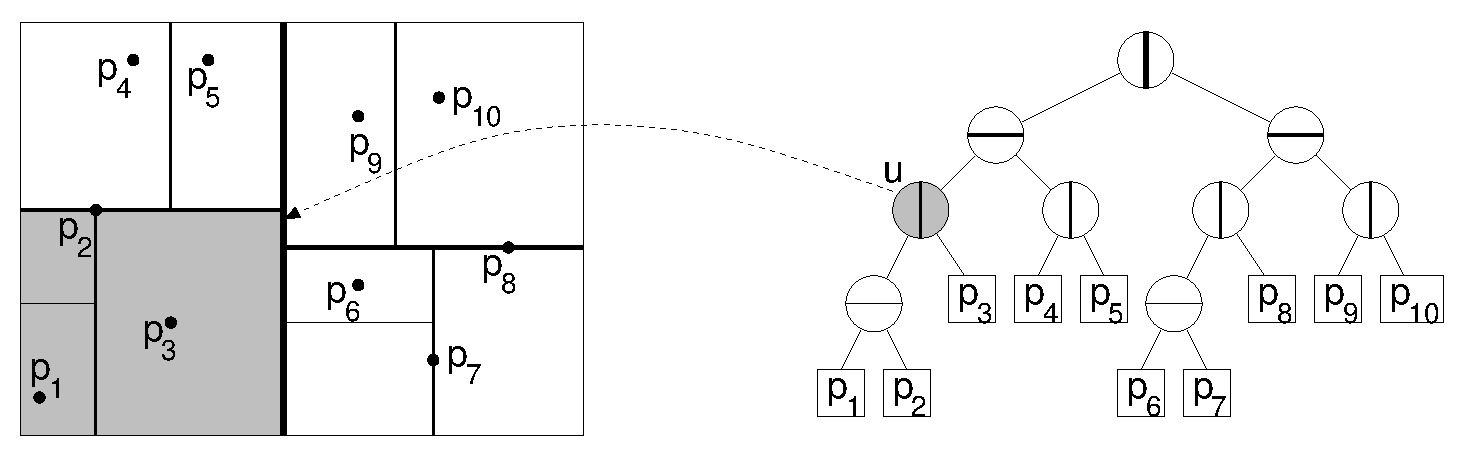
\includegraphics[height=1.5in]{Figs/kd-tree.eps}}
  \caption{A kd-tree of bucket-size one and the corresponding spatial
  decomposition.}
  \label{kd-tree.fig}
\end{figure}

These two boxes are the cells associated with the two children of this
node.  The data points lying in the original box are split between these
two children, depending on which side of the splitting hyperplane they
lie.  Points lying on the hyperplane itself may be associated with either
child (according to the dictates of the splitting rule).  When the number
of points that are associated with the current box falls below the bucket
size, then the resulting node is declared a \emph{leaf node}, and these
points are stored with the node.

The problem with the splitting operation used in kd-trees is that, when
points are highly clustered, it may either take many splits to partition
these points or the splits may result is highly elongated boxes (which can
be problematic when searching is performed).  {\ANN} supports the bd-tree
data structure to provide greater robustness for highly clustered data
sets.  The bd-tree is a variant of the data structure described in
\cite{AMN98}.  It differs from the kd-tree mainly in that, in addition
to the splitting operation, there is a more general decomposition operation
called \emph{shrinking}.  As above, consider a node whose associate box
$B$ contains more points than the bucket size.  A \emph{shrinking rule}
is then invoked.  This rule may opt to simply defer and perform a split
according to the prevailing splitting rule.  Otherwise, it selects an
axis-aligned box $B'$ lying within $B$.  The points lying inside $B'$
are associated with one child and the points lying outside $B'$ are
associated with the other child.  As before, points lying on the boundary
of $B'$ may be associated with either child.

Thus, in addition to the data points themselves, a kd-tree is specified by
two additional parameters, the bucket size and a splitting rule.  A
box-decomposition tree is defined by these two parameters as well, and an
additional parameter, the shrinking rule.  {\ANN} provides a number of
different splitting rules and shrinking rules.  It also provides
reasonable default values for these parameters.

The (almost) complete prototypes for the constructors for kd-trees and
bd-trees are given below.  Refer back to Section~\ref{struct.sec} for
definitions of the data point array $pa$, number of points $n$, and
dimension $d$.  The types \textsf{ANNsplitRule} and \textsf{ANNshrinkRule}
are splitting rules and shrinking rules.  They are described in later
sections.

{\small \begin{verbatim}
    enum ANNsplitRule {                     // splitting rules for kd-trees
            ANN_KD_STD,                     // standard kd-splitting rule
            ANN_KD_MIDPT,                   // midpoint split
            ANN_KD_FAIR,                    // fair-split
            ANN_KD_SL_MIDPT,                // sliding midpoint split
            ANN_KD_SL_FAIR,                 // sliding fair-split
            ANN_KD_SUGGEST};                // the authors' suggestion for best

    enum ANNshrinkRule {                    // shrinking rules for bd-trees
            ANN_BD_NONE,                    // no shrinking at all (just kd-tree)
            ANN_BD_SIMPLE,                  // simple splitting
            ANN_BD_CENTROID,                // centroid splitting
            ANN_BD_SUGGEST};                // the authors' suggested choice
        
    ANNkd_tree(                             // build a kd-tree from a point array
            ANNpointArray   pa,             // point array
            int             n,              // number of points
            int             d,              // dimension
            int             bs = 1,         // bucket size
            ANNsplitRule    split = ANN_KD_SUGGEST);        // splitting rule

    ANNbd_tree(                             // build a bd-tree from a point array
            ANNpointArray   pa,             // point array
            int             n,              // number of points
            int             d,              // dimension
            int             bs = 1,         // bucket size
            ANNsplitRule    split  = ANN_KD_SUGGEST,        // splitting rule
            ANNshrinkRule   shrink = ANN_BD_SUGGEST);       // shrinking rule
\end{verbatim} }

% There are additional arguments which may be passed to the constructors
% when subsequent point insertion is desired.  These are described in
% Section~\ref{insert.sec}.

\subsubsection{Internal Tree Structure}\label{intern.sec}

Before discussing the various splitting and shrinking rules, we digress
to discuss the internal structure of these two trees.  This material is
not needed for using the data structures, but it provides some
background for understanding how the search algorithms work.

The root structure for both kd- and bd-trees contains the same
information.  It contains global information such as the number of
points $n$, the dimension of the space $d$, and the bucket size, $b$.
It does not store the points, but rather maintains a pointer to the
array $pa$ of data points given in the constructor.  It allocates an
$n$-element array $\it pidx$ of point indices.  It also stores a
bounding hyperrectangle that contains all the data points, and a pointer
to the root of the kd- or bd-tree.

A leaf node in either type of tree stores the number of points that are
associated with this node (which ranges from 0 up to the bucket size)
and an array of point indices.  This point index array is actually a
subarray of \textit{pidx}.

A splitting node in a kd-tree contains the following information.
First, it stores the integer \emph{cutting dimension} (from 0 to $d-1$)
indicating the coordinate axis that is orthogonal to the cutting
hyperplane.  Second it stores the \emph{cutting value} where this plane
intersects this axis.  It also contains the two pointers to the left and
right children (containing points lying to the low and high side of the
cutting plane, respectively).  The search algorithm uses a technique
called \emph{incremental distance computation} \cite{ArM93b} for
speeding up the computation of distances between the query point and the
associated cells of nodes of the tree.  In order to implement
incremental distance computation, it also stores two associated pieces
of information with the cell.  Consider the two hyperplanes bounding the
cell that are parallel to the cutting plane.  It stores the values at
which these two hyperplanes intersect the cutting dimension's axis.

Leaf and splitting nodes in a bd-tree contain exactly the same
information as in the kd-tree.  The only difference is that the tree may
also contain shrinking nodes.  A shrinking node consists of a set of at
most $2d$ orthogonal halfspaces.  Each orthogonal halfspace is
represented by storing a cutting dimension, a cutting value (which
together define an orthogonal hyperplane), and an integer $-1$ or $+1$,
which indicates to which side (negative or positive, respectively) of
this plane the halfspace lies.  The node contains the number of
orthogonal halfspaces bounding the inner box, and an array of these
halfspaces.  (The reason for not storing all $2d$ bounding halfspaces is
that in high dimensional applications, the shrinking node may only
involve a relatively small number of halfspaces.)

\subsubsection{Splitting Rules for kd-trees}\label{splitrule.sec}

This section describes the various splitting rules for kd-trees that are
supported by {\ANN}.  Let $S$ denote the current subset of data points to
be stored in the tree, let $n$ denote the number of points in $S$, let
$C$ denote the current cell.  Let $R(C)$ denote the bounding rectangle
for the current cell.  The points of $S$ are all contained in $R(C)$.
Let $R(S)$ denote the bounding rectangle for $S$.   This rectangle is
contained within (and may be equal to) $R(C)$.  Initially, $S$ is the set of
all data points, and $C$ is the root of the kd-tree, and $R(C)$ is the
enclosing bounding rectangle for $S$.  Define the \emph{aspect ratio} of
a rectangle to be the ratio between its longest and shortest side lengths.
Given a dimension, define the \emph{point spread} of $S$ along this
dimension to be the difference between the largest and smallest coordinate
for this dimension.  This is equivalent to the longest side of $R(S)$.

Given a set of numbers $A$, a \emph{median partition} of the $n$ numbers
is a partition of $A$ into two subsets, one with $\floor{n/2}$ elements
whose values are no greater than the median of $A$, and the other with
$\ceil{n/2}$ elements whose values are no less than the median of $A$.

\begin{description}
    
\item[\hbox{\sf ANN\_KD\_STD:}]
	This is called the \emph{standard kd-tree splitting rule}.
	The splitting dimension is the dimension of the maximum spread
	of $S$.  The splitting point is the median of the coordinates of $S$
	along this dimension.  A median partition of the points $S$ is
	then performed.  This rule guarantees that the final tree has height
	$\ceil{\log_2 n}$, and size $O(n)$, but the resulting cells may have
	arbitrarily high aspect ratio.

\item[\hbox{\sf ANN\_KD\_MIDPT:}]
	This is a simple splitting rule, which guarantees that cells have
	bounded aspect ratio, and is called the \emph{midpoint splitting
	rule}.  It simply cuts the current cell through its midpoint orthogonal
	to its longest side.  It can be seen as a binary variant of a quad tree,
	since with every $d$ levels of the tree, a hypercube of side length $x$
	is partitioned into equal hypercubes of side length $x/2$ each.  If
	there are ties, it selects the dimension with the maximum point spread.
	
	This rule can produce \emph{trivial splits}, meaning that all of the
	points of $S$ lie to one side of the splitting plane.  As a result, the
	depth of and size of the resulting tree can be arbitrarily large, and
	both may even exceed $n$ if the points are highly clustered.

\item[\hbox{\sf ANN\_KD\_SL\_MIDPT:}]
	This is a simple modification of the midpoint
	splitting rule, called the \emph{sliding-midpoint rule}.  It first
	attempts to perform a midpoint split, by the same method described
	above.  If points of $S$ lie on both sides of the splitting plane
	then the algorithm acts exactly as it would for the midpoint split.

	However, if a trivial split were to result, then it attempts to
	avoid this by ``sliding'' the splitting plane toward the points until
	it encounters the first data point.  More formally, if the split is
	performed orthogonal to the $i$th coordinate, and all the points of $S$
	have $i$-coordinates that are larger than that of the splitting plane,
	then the splitting plane is translated so that its $i$th coordinate
	equals the minimum $i$th coordinate among all the points of $S$.  Let
	this point be $p_1$.  Then the points are partitioned with $p_1$ in
	one part of the partition, and all the other points of $S$ in the other
	part.  A symmetrical rule is applied if the points all have $i$th
	coordinates smaller than the splitting plane.

	This rule cannot result in any trivial splits, implying that the
	tree has maximum depth $n$ and size $O(n)$.  It is possible to
	generate a cell $C$ of very high aspect ratio, but it can be shown
	that if it does, then $C$ is necessarily adjacent to a sibling cell
	$C'$ that is fat along the same dimension that $C$ is skinny.  It
	turns out that cells of high aspect ratio are not problematic for
	nearest neighbor searching if this occurs.

\item[\hbox{\sf ANN\_KD\_FAIR:}]
	This is a compromise between the standard kd-tree
	splitting rule (which always splits data points at their median)
	and the midpoint splitting rule (which always splits a box through
	its center.  It is called the \emph{fair-split rule}.  The goal of
	this rule is to achieve as nicely balanced a partition as possible,
	provided that the aspect ratio bound is never violated.

	A constant \textsf{FS\_ASPECT\_RATIO = 3} is defined in the source
	file \textsf{src/kd\_split.cpp}.  Given a cell, it first determines
	the sides of this cell that can be split in some way so that the
	ratio of the longest to shortest side does not exceed
	\textsf{FS\_ASPECT\_RATIO} are identified.  Among these sides, it
	selects the one in which the points have the largest spread.  It
	then splits the points in the most even manner possible, subject
	to maintaining the bound on the ratio of the resulting cells.  To
	determine that the aspect ratio will be preserved, we determine
	the longest side (other than this side), and determine how narrowly
	we can cut this side, without causing the aspect ratio bound to
	be exceeded.

	This procedure is more robust than either the kd-tree splitting rule
	or the pure midpoint splitting rule when data points are highly
	clustered.  However, like the midpoint splitting rule, if points
	are highly clustered, it may generate a large number of trivial
	splits, and may generate trees whose size exceeds $O(n)$.

\item[\hbox{\sf ANN\_KD\_SL\_FAIR:}]
	This rule is called \emph{sliding fair-split}.  It is a splitting rule
	that is designed to combine the strengths of both fair-split with
	sliding midpoint split.  Sliding fair-split is based on the theory
	that there are two types of splits that are good: balanced splits
	that produce fat boxes, and unbalanced splits provided the cell
	with fewer points is fat.

	This splitting rule operates by first computing the longest side of
	the current bounding box.  Then it asks which sides could be split
	and still satisfy the aspect ratio bound with respect to this side.
	Among these, it selects the side with the largest spread (just as
	fair-split would).  It then considers the most extreme cuts that
	would be allowed by the aspect ratio bound.  This is done by
	dividing the longest side of the box by the aspect ratio bound.
	If the median cut lies between these extreme cuts, then we use the
	median cut.  If not, then consider the extreme cut that is closer
	to the median.  If all the points lie to one side of this cut, then
	we slide the cut until it hits the first point.  This may violate
	the aspect ratio bound, but will never generate empty cells.
	However the sibling of every such skinny cell is fat, as with
	sliding midpoint split.

\item[\hbox{\sf ANN\_KD\_SUGGEST:}]
	This is the default splitting rule.  It is set to the splitting
	rule which, in the authors' opinion, performs best with typical
	data sets.  It is currently set to \textsf{ANN\_KD\_SL\_MIDPT}, the
	sliding midpoint rule.
\end{description}

\subsubsection{Shrinking Rules for bd-trees}\label{shrinkrule.sec}

This section describes the various shrinking rules for bd-trees that are
supported by {\ANN}.  Let $S$, $C$, and $n$, be the same as defined in the
previous section and let $d$ denote the dimension

{\ANN} first attempts to perform shrinking.  Each of shrinking rules have the
option of electing to not shrink.  If this is the case, then processing is
passed to the current splitting rule instead.

\begin{description}
\item[\hbox{\sf ANN\_BD\_NONE:}] When this rule is selected, no shrinking is
	performed at all, only splitting.  A bd-tree generated with this
	shrinking rule is identical to a kd-tree.

\item[\hbox{\sf ANN\_BD\_SIMPLE:}]
	This is called a \emph{simple shrink}.  It depends on two constants:
	\textsf{BD\_GAP\_THRESH} whose value is $0.5$,  and
	\textsf{BD\_CT\_THRESH} whose value is 2.  It first computes the
	tight bounding box of the points, and computes the $2d$ \emph{gaps},
	that is, the distances between each side of the tight enclosing
	rectangle for the data points $R(S)$ and the corresponding side of
	the cell's bounding rectangle $R(C)$.  If at least
	\textsf{BD\_CT\_THRESH} of the gaps are larger than the length the
	longest side of $R(S)$ times \textsf{BD\_GAP\_THRESH}, then it
	shrinks all sides whose gaps are at least this large.  After the
	shrink has been performed, all of the points of $S$ lie in the inner
	box of the shrink, and the outer box contains no points.  If none of
	the gaps is large enough, then no shrinking is performed, and
	splitting is performed instead.

\item[\hbox{\sf ANN\_BD\_CENTROID:}]

	This rule is called a \emph{centroid shrink}.  Its operation depends
	on two constants: \textsf{BD\_MAX\_SPLIT\_FAC} and
	\textsf{BD\_FRACTION}, both of whose value are $0.5$.  It repeatedly
	applies the current splitting rule (without actually generating new
	cells in the tree).  In each case we see which half of the partition
	contains the larger number of points, and we repeat the splitting on
	this part.  This is repeated until the number of points falls below
	a fraction of \textsf{BD\_FRACTION} of the original size of $S$.  If
	it takes more than \textsf{dim*BD\_MAX\_SPLIT\_FAC} splits for this
	to happen, then we shrink to the final inner box.  All the other
	points of $S$ are placed in the outer box.  Otherwise, shrinking is
	not performed, and splitting is performed instead.

\item[\hbox{\sf ANN\_BD\_SUGGEST:}]
	This is the default shrinking rule.  It is set to the shrinking rule
	which, in the authors' opinion, performs best in most circumstances.
	It is currently set to \textsf{ANN\_BD\_SIMPLE}.
\end{description}

%----------------------------------------------------------------------
\subsection{Search Algorithms}\label{search.sec}
%----------------------------------------------------------------------

{\ANN} supports two different methods for searching both kd- and bd-trees.
The first is called \emph{standard search}.  It is the simpler of
the two methods, and visits cells in order based on the hierarchical
structure of the search tree.  The second method, called \emph{priority search},
visits cells in increasing order of distance from the query point, and
hence, should converge more rapidly on the true nearest neighbor.  However,
priority search requires the use of a heap, and so has a somewhat higher
overhead.  When the error bound is small, standard search seems to be
slightly faster.  When larger error bounds are used, or when early
termination is used (described in Section~\ref{term.sec} below) then
priority search seems to be superior.

\subsubsection{Standard Search}\label{stdsearch.sec}

Standard search is an adaptation of the search algorithm described by
Friedman, Bentley, and Finkel \cite{FBF77}, but for approximate nearest
neighbor searching.  The algorithm operates recursively.  When first
encountering a node of the kd-tree the algorithm first visits the child
that is closest to the query point.  On return, if the box containing
the other child lies within $1/(1+\epsilon)$ times the distance to the
closest point seen so far, then the other child is visited recursively.
The distance between a box and the query point is computed exactly (not
approximated), using incremental distance updates, as described by Arya
and Mount \cite{ArM93b}.

The search is similar for bd-trees.  For shrinking nodes we compute the
distances to the inner box and the outer box and recurse on the closer.
In case of a tie, we favor the inner box.

The prototype is given below.  The argument $q$ is the query point, $k$
is the number of nearest neighbors, to return \textit{nn\_idx} is an
array of at least $k$ point indices, and $\it dists$ is an array of at
least $k$ elements of type \textsf{ANNdist}, and $\it eps$ is the
(optional) error bound in nearest neighbor searching.  If $\it eps$ is
omitted or zero, then the $k$ nearest neighbors are computed exactly.
The $k$ (approximate) nearest neighbor squared distances are stored in
the elements of $\it dists$, and the indices of the nearest neighbors
are returned in the elements of $\it nn\_idx$.  An error results if $k$
exceeds the number of data points.  The next two sections describe the
search algorithms in greater detail.

{\small \begin{verbatim}
    virtual void annkSearch(            // standard search
        ANNpoint        q,              // query point
        int             k,              // number of near neighbors to return
        ANNidxArray     nn_idx,         // nearest neighbor array (returned)
        ANNdistArray    dists,          // dists to near neighbors (returned)
        double          eps=0.0);       // error bound
\end{verbatim} }


\subsubsection{Priority Search}\label{prsearch.sec}

Priority search is described by Arya and Mount \cite{ArM93}.  The cell of
the kd-tree containing the query point is located, and cells are visited in
increasing order of distance from the query point.  This is done as follows.
Whenever we arrive at a nonleaf node, we compute the distances from the
query point to the cells of the two children.  We enqueue the further
child on a priority queue, sorted by distance, and then visit the closer
child recursively.  On arriving at a leaf node, we compute the distances
to the points stored in this node, and continue by dequeing the next
item from the priority queue.  The search stops either when the priority
queue is empty (meaning that the entire tree has been searched) or when the
distance to the nearest cell on the priority queue exceeds the distance to
the nearest point seen by a factor of more than $1/(1+\epsilon)$.

The search is similar for bd-trees.  For shrinking nodes we compute the
distances to the inner box and to the outer box.  We visit the closer one
and enqueue the further, breaking ties in favor of the inner box.  (Note
that this differs slightly from the description in \cite{AMN98}.  There
the cell of the outer child is the set theoretic difference between the
inner box and the outer box, implying a more complex distance computation.)
The prototype for both trees is essentially the same as that of the standard
search, described above.

A priority-search variant of \textsf{annkSearch()} is provided, and the
prototype is given below.  There is no priority-search variant of
the fixed-radius search, \textsf{annkFRSearch()}.

{\small \begin{verbatim}
    virtual void annkPriSearch(         // priority search
        ANNpoint        q,              // query point
        int             k,              // number of near neighbors to return
        ANNidxArray     nn_idx,         // nearest neighbor array (returned)
        ANNdistArray    dists,          // dists to near neighbors (returned)
        double          eps=0.0);       // error bound
\end{verbatim} }

\subsubsection{Early Termination Option}\label{term.sec}

In situations where response time is critical, the search algorithm
(either standard or priority search) can be forced to terminate prior to
the normal termination conditions described earlier.  This is done by
invoking the function \textsf{annMaxPtsVisit()}.  The single integer
argument is the maximum number of points that the search algorithm will
visit before terminating.  The algorithm maintains a count of the number
of points visited, and tests this quantity before visiting each leaf
node.  Since the test is only made prior to visiting each leaf, it may
visit some additional points depending on the bucket size.

The bound remains in effect until it is changed by a subsequent call to
this function.  To disable early termination, call the function
with the argument 0.  This is not a member function, but a free-standing
procedure, which sets a global variable.  Thus, if there are two search
structures to which queries are being performed, and different maximum
point values are desired for each, then it would be necessary to call
this function prior to switching between the structures.

{\small \begin{verbatim}
    void annMaxPtsVisit(
        int                 maxPts);
\end{verbatim} }

If this bound is set, the neraest neighbor search procedures may
terminate before all of the $k$ nearest neighbors have been encountered.
Therefore, this function should be invoked with care.

%----------------------------------------------------------------------
\subsection{Search Tree Utility Functions}\label{utilproc.sec}
%----------------------------------------------------------------------

{\ANN} provides a number of utility member functions for gathering statistics
on kd-trees and bd-trees, printing the tree in a format suitable for
reading, and dumping the tree for the purpose of reading it by another
program.  Since they are member functions, they are invoked in essentially
the same way as is the \textsf{annkSearch} procedure.

\subsubsection{Printing the Search Structure}\label{print.sec}

The procedure Print is used to print the contents of a kd- or bd-tree
in a format that is suitable for reading.  This is provided primarily
for debugging purposes. This procedure prints the nodes of the
tree according to a right-to-left inorder traversal.  That is, for
an internal node it first prints the high (or outer) child, then the
node itself, then the low (or inner) child.  (This is done this way
because by tilting the output clockwise, the traversal appears to be
left to right.)

For each leaf, it prints the number of points associated with the leaf,
and for each point it outputs the index of the point.  For each splitting
node, it outputs the cutting dimension ($cd$), the cutting value ($cv$),
the low bound ($\it lbnd$), and the high bound ($\it hbnd$) for the node.
For shrinking nodes it prints the set of bounding halfspaces, two per
line.  For each bounding halfspace it prints the cutting dimension,
the cutting value, and indicates whether the inner box lies on the greater
or lesser side of the cutting value.

The level of the node in the tree is indicated by its indentation in the
output.  If the boolean \textit{with\_pts} argument is true, then the data
coordinates points are printed before the tree, otherwise they are not
printed.  The other argument is the output stream to which the output is
sent.

{\small \begin{verbatim}
    void Print(                         // print the tree (for debugging)
        ANNbool         with_pts,       // print points as well?
        ostream&         out);          // output stream
\end{verbatim} }

\subsubsection{Saving and Restoring the Search Structure on a File}\label{dump.sec}

The member function \textsf{Dump()} copies a kd- or bd-tree and the associated
points to a stream.  (It is currently not provided from the brute-force
data structure.) The tree is printed in preorder, first printing each node,
then the low (or inner) child, followed by the high (or outer child).  This
output format is not intended for human reading, but instead for saving the
data structure for the purposes of loading it later, or for consumption
by another program (such as {\annfig}), for analysis of the tree.

As with Print, the first argument indicates whether the points are to be
printed, and the second argument is the output stream to which the
output is sent.

{\small \begin{verbatim}
    void Dump(                          // dump entire tree
        ANNbool         with_pts,       // print points as well?
        ostream&         out);          // output stream
\end{verbatim} }

To restore a saved structure, there is a constructor, which is given an
input stream, which is assumed to have been created through the \textsf{Dump()}
function, and creates a search structure from the contents of this file.
It is assumed that the file was saved with the points printed.

{\small \begin{verbatim}
    ANNkd_tree(                         // build structure from a dump file
        istream&         in);           // input stream for dump file
\end{verbatim} }

For example, to save the current structure \textsf{the\_tree} to ostream
\textsf{foo} and then load a new structure from istream \textsf{bar} the
following could be used.

{\small \begin{verbatim}
    ANNkd_tree* the_tree = new ANNkd_tree(...);
    the_tree->Dump(ANNtrue, foo);       // save the current tree contents
    delete the_tree;                    // deallocate (to prevent memory leaks)
    // ... (sometime later)
    the_tree = new ANNkd_tree(bar);     // restore a copy of the old tree
\end{verbatim} }

The dump output format consists of the following elements.  All entries
on a line are separated by white space.

\begin{description}
\item[Header:] A line containing \textsf{\#ANN} followed the version number
	for {\ANN}.
\item[Points:] If the parameter \textit{with\_pts} is true, then this section
	is printed.  It starts with a line beginning with the word
	\textsf{points}, followed by the dimension of the space $d$, and the
	number of points $n$.  This is then followed by $n$ lines, each
	containing the integer index of the point, followed by the $d$
	coordinates of the point.  One issue for floating point data is
	the desired output precision.  This is stored in the variable
	\textsf{ANNcoordPrec} in the file \textsf{include/ANN/ANN.h}.
\item[Tree Structure:] The tree structure describes the tree contents.
	It begins with a single header entry followed by a series of
	entries, one for each node of the tree, given according to a
	preorder traversal of the tree, as described above.  There is
	no distinction made between kd-trees and bd-trees, except that
	kd-trees have no shrinking nodes.
	\begin{description}
	\item[Header:] This starts with a line containing the word \textsf{tree},
		followed by the dimension $d$, the number of points $n$, and
		the bucket size $b$.  This is followed by 2 lines, giving
		the lower endpoint and upper endpoint of the bounding box
		of the tree's root cell.
	\item[Leaf node:] The starts with the word \textsf{leaf} followed by
		the number of points $m$ stored in this leaf (from 0 to
		$b$), followed by the $m$ integer indices of these points.
	\item[Splitting node:] Starts with the word \textsf{split} followed by
		the cutting dimension, cutting value, lower bound and
		upper bound for the node.
	\item[Shrinking node:] Starts with the word \textsf{shrink} followed
		by the number of bounding sides $m$, followed by $m$ lines,
		each containing a cutting dimension, cutting value, and
		the side indicator ($1$ or $-1$), for this bounding side.
	\end{description}
\end{description}

\subsubsection{Gathering Statistics on Tree Structure}

The procedure getStats computes statistics on the shape and properties
of the search tree.  These are returned in the structure \textsf{ANNkdStats}.
This is something of a misnomer, because the stats apply to both kd-trees
and bd-trees.  This structure is returned (as the argument) to the
following procedure.

{\small \begin{verbatim}
    void getStats(                      // compute tree statistics
        ANNkdStats&      st);           // the statistics (returned)
\end{verbatim} }

The statistics structure contains the following public members, which
are all set by the call to \textsf{getStats}.  The total number of
leaves is stored in \textsf{n\_lf}. In order to save space, {\ANN}
distinguishes between leaves that do and do not contain points.  Leaves
that contain no points are called \emph{trivial leaves}, and are counted
in \textsf{n\_tl}.  (Because some splitting rules may generate a large
number of trivial leaves, {\ANN} saves space by storing just one
\emph{canonical} trivial leaf cell, and each trivial leaf generated by
the algorithm is implemented by a single pointer to this canonical
cell.)

Internal nodes are of two types, splitting nodes and shrinking nodes.
The former is counted in \textsf{n\_spl} and the latter in
\textsf{n\_shr}.  Since kd-trees do not perform shrinking, the value of
\textsf{n\_shr} is nonzero only for bd-trees.  The maximum depth of the
tree is stored in \textsf{depth}.  The \emph{aspect ratio} of a leaf
cell is the ratio between the lengths of its longest and shortest sides.
There is theoretical evidence that nearest neighbor searching is most
efficient when the aspect ratio is relatively small (say, less than 20).
The average aspect ratio of all the leaf cells is stored in
\textsf{avg\_ar}.

{\small \begin{verbatim}
    class ANNkdStats {                  // stats on kd-tree
    public:
        int dim;                        // dimension of space
        int n_pts;                      // number of points
        int bkt_size;                   // bucket size
        int n_lf;                       // number of leaves
        int n_tl;                       // number of trivial leaves
        int n_spl;                      // number of splitting nodes
        int n_shr;                      // number of shrinking nodes (bd-trees only)
        int depth;                      // depth of tree
        float avg_ar;                   // average leaf aspect ratio
    }
\end{verbatim} }

%----------------------------------------------------------------------
\subsection{Compile-Time Options}\label{compileopt.sec}
%----------------------------------------------------------------------

{\ANN} contains a number of options that are activated when the program
is compiled.  These are activated or deactivated by adding these
parameters to the ``\textsf{CFLAGS}'' variable in the file
\textsf{Make-config}, before compiling the library.  For example:
\begin{verbatim}
      "CFLAGS = -O3 -Wall -DANN_PERF"
\end{verbatim}
Some of these options are described below (see \textsf{Make-config} for
others). By default, none of these are active, except the ``-O'' for
optimization.

\begin{description*}
\item[\hbox{\sf -O:}] (or ``\textsf{-O3}'') Produce code optimized for
	execution speed.
\item[\hbox{\sf -DANN\_PERF:}] This causes code to be compiled that
	performs additional performance measurements on the efficiency of
	the structure (e.g., the average CPU time per query). Setting this
	option can slow execution by around 10\%.
\item[\hbox{\sf -DANN\_NO\_LIMITS\_H:}] Use this if your system does
	not have either of the include files $\ang{\textsf{limits.h}}$ or
	$\ang{\textsf{float.h}}$, which are needed for the definition of
	system-dependent quantities like \textsf{DBL\_MAX}. (Also see
	\textsf{include/ANN/ANN.h} for other changes that may be needed.)
\item[\hbox{\sf -DANN\_NO\_RANDOM:}] Use this if your system does
	not support the built-in pseudo-random number generators
	\textsf{srandom()} or \textsf{random()}.  Pseudo-random number
	generation is used in the utility program \textsf{test/ann\_test}.
	(It is not required if you just want to compile the {\ANN} library.)
	Virtually all C++ systems provide a simple pseudo-random number in
	the form of two build-in functions \textsf{srand()} and
	\textsf{rand()}.  However, these functions are inferior to the less
	widely available functions \textsf{srandom()} and \textsf{random()}.
	By setting this option, the program will use functions
	\textsf{srand()} and \textsf{rand()} instead.  This is needed on
	most Microsoft Visual C++ systems.
\end{description*}

%----------------------------------------------------------------------
\newpage
\section{Utility Programs}
%----------------------------------------------------------------------

As mentioned earlier, {\ANN} is not just a library for nearest neighbor
searching, but it is also provides a testbed for nearest neighbor data
structures and algorithms.  There are two utility programs provided
with {\ANN} for the purpose of evaluating and visualizing search structures
(under various splitting and shrinking rules) for a number of different
data distributions.  These are {\anntest} and {\annfig},
described in the following sections.  If you are just interested in the
{\ANN} library, you do not need to compile these two programs.

%----------------------------------------------------------------------
\subsection{\anntest: A Test and Evaluation Program}\label{anntest.sec}
%----------------------------------------------------------------------

The program {\anntest} provides a simple script language for setting up
experiments involving {\ANN}.  It allows the user to generate data and
query sets of various sizes, dimensions, and distributions, to build kd-
and bd-trees of various types, and then run queries and outputting
various performance statistics.

The program reads commands from the standard input and writes its
results to the standard output.  The input consists of a sequence of
\emph{directives}, each consisting of a directive name, followed by list
of 0 or more arguments (depending on the directive).  Arguments and
directives are separated by white space (blank, tab, and newline).
String arguments are not quoted, and consist of a sequence of nonwhite
characters.  The character ``\#'' denotes a comment.  The following
characters up to the end of line are ignored.  Comments may only be
inserted between directives (not within the argument list of a
directive).

Directives are of two general types: \emph{operations}, which cause some
action to be performed and \emph{parameter settings}, which set the
values of various parameters that affect later operations.  As each line
of the input file is read, the appropriate operation is performed or the
appropriate parameter value is set.  For example, to build a kd-tree
with a certain splitting rule, first set the parameter that controls the
splitting rule, and then invoke the operation for building the tree.

A number of the operations (particularly those involving data generation)
involve generation of pseudo-random numbers.  The pseudo-random number
generator can be controlled by an integer \emph{seed} parameter.  Once
the seed is set, the subsequent sequence of pseudo-random numbers is
completely determined.  For example, to generate identical but pseudo-random
data point sets and query point sets, first set the seed to some desired
value, issue the operation to generate the data points, then reset the
seed to this same value, and then issue the operation to generate the
query points.

The following section lists the basic operations (directives that perform
actions), and the remaining sections describe various parameters that
affect how these operations are performed.  Arguments and their type are
indicated with angled brackets.  For example \STRING\ means that the
argument is a character string.  String and filename arguments consist
of a sequence of characters with no embedded whitespaces (blank, tab,
or newline).  No quoting is needed (nor is it allowed).  Currently there
is no facility for placing comments within the script file.

\subsubsection{Operations}

\begin{description}
\item[\hbox{\sf output\_label \STRING:}]
	Prints the string to the output file.
\item[\hbox{\sf gen\_data\_pts:}]
	Generates a set of pseudo-random data points.  The number of points
	is determined by the \textsf{data\_size} parameter, the number of
	coordinates is determined by the \textsf{dim} parameter, and the point
	distribution is determined by the \textsf{distribution} parameter.
	Data points generated by an earlier call to this operation or the
	\textsf{read\_data\_pts} operation are discarded.  Relevant parameters:
	\textsf{data\_size}, \textsf{dim}, \textsf{std\_dev}, \textsf{corr\_coef},
	\textsf{colors}, \textsf{seed}, and \textsf{distribution}.
\item[\hbox{\sf gen\_query\_pts:}]
	Same as \textsf{gen\_data\_pts} but for the current query point set.
	Relevant parameters: \textsf{data\_size}, \textsf{dim}, \textsf{std\_dev},
	\textsf{corr\_coef}, \textsf{colors}, \textsf{seed}, and \textsf{distribution}.
\item[\hbox{\sf read\_data\_pts \FILE:}]
	Reads a set of data points from the given file.  Each point consists
	of a sequence of \textsf{dim} numbers (of type \textsf{ANNcoord}) separated
	by whitespace (blank, newline, or tab).  It is assumed that the
	file contains no more points than given by the \textsf{data\_size}
	parameter, otherwise only this many points of the data set are input.
	Relevant parameters: \textsf{data\_size}, \textsf{dim}.
\item[\hbox{\sf read\_query\_pts \FILE:}]
	Same as \textsf{read\_data\_pts} but for the current query point set.
	The parameter \textsf{query\_size} indicates the maximum number of
	points.  Relevant parameters: \textsf{query\_size}, \textsf{dim}.
\item[\hbox{\sf build\_ann:}] Builds either a kd-tree or bd-tree for the
	current data point set according to current splitting rule (see
	the \textsf{split\_rule} parameter) and shrinking rule (see
	\textsf{shrink\_rule}).  If the shrinking rule is ``none'' then a
	kd-tree results, and otherwise a bd-tree results.  Relevant
	parameters: \textsf{split\_rule}, \textsf{shrink\_rule}.
\item[\hbox{\sf run\_queries \STRING:}]
	Apply nearest neighbor searching to the current query point set
	using the current approximate nearest neighbor structure (resulting
	from \textsf{build\_ann}, for the current number of nearest neighbors
	(see \textsf{near\_neigh}), and the current error bound (see
	\textsf{epsilon}), and with the search strategy specified in the
	argument.  Possible strategies are:
	\begin{description}
	\item[\hbox{\sf standard:}]
		Standard search.  (See Section~\ref{stdsearch.sec}.)
	\item[\hbox{\sf priority:}]
		Priority search.  (See Section~\ref{prsearch.sec}.)
	\end{description}
	Relevant parameters: \textsf{epsilon}, \textsf{near\_neigh},
	\textsf{max\_pts\_visit}.
\item[\hbox{\sf dump \FILE:}]
	Dump the current search structure to the specified file.  See
	Section~\ref{dump.sec}.  If the dump file is to be read by the
	{\annfig} program, then the file name should end with the suffix
	``.dmp''.
\item[\hbox{\sf load \FILE:}]
	Loads a tree from a data file that was created by the dump
	operation.	Any existing tree structure and data point storage
	will be deallocated.
\end{description}

\subsubsection{Options Affecting Tree Structure:}

\begin{description}
\item[\hbox{\sf split\_rule \STRING:}]
	Type of splitting rule to use in building a kd-tree or bd-tree.
	Choices are as follows. See Section~\ref{splitrule.sec} for
	further information.
	\begin{description}
	\item[\hbox{\sf standard:}] Perform standard optimized kd-tree
			splitting.
	\item[\hbox{\sf midpt:}] Perform midpoint splitting.
	\item[\hbox{\sf fair:}] Perform fair-split splitting.
	\item[\hbox{\sf sl\_midpt:}] Perform sliding midpoint splitting.
	\item[\hbox{\sf sl\_fair:}] Perform sliding fair-split splitting.
	\item[\hbox{\sf suggest:}]	Perform the authors' suggested choice for the
		best splitting rule.  (Currently \textsf{sl\_midpt}.)
	\end{description}
	Default: \textsf{suggest}.
\item[\hbox{\sf shrink\_rule \STRING:}]
	Specifies the type of shrinking rule to use in building a bd-tree
	data structure.  If \textsf{none} is specified, then no shrinking is
	performed and the result is a kd-tree.  Choices are as follows.
	See Section~\ref{shrinkrule.sec} for further information.
	\begin{description}
	\item[\hbox{\sf none:}] Perform no shrinking.
	\item[\hbox{\sf simple:}] Perform simple shrinking.
	\item[\hbox{\sf centroid:}] Perform centroid shrinking.
	\item[\hbox{\sf suggest:}] Perform the authors' suggested choice for best.
		(Currently \textsf{none}.)
	\end{description}
	Default: \textsf{none}.
\item[\hbox{\sf bucket\_size \INT:}]
	Bucket size, that is, the maximum number of points stored in each
	leaf node of the search tree.  Bucket sizes larger than 1 are
	recommended for the ``midpt'' splitting rule when the dimension is 3
	or higher. It is also recommended when performance evaluation shows
	that there are a large number of trivial leaf cells. Default: 1.
\end{description}

\subsubsection{Options Affecting Data and Query Point Generation}

The test program generates points according to the following probability
distributions.
\begin{description}
\item[\hbox{\sf uniform:}] Each coordinate is chosen uniformly from the interval
	$[-1,1]$.
\item[\hbox{\sf gauss:}] Each coordinate is chosen from the Gaussian distribution
	with the current standard deviation (see \textsf{std\_dev}) and
	mean 0.
\item[\hbox{\sf clus\_gauss:}]
        Some number of cluster centers (set by the parameter \textsf{colors}
	below) are chosen from the above uniform distribution.  Then
	each point is generated by selecting a random cluster center, and
	generating a point with a Gaussian distribution with the current
	standard deviation (see \textsf{std\_dev}) centered about this cluster
	center.

	Note that once the cluster centers have been set, they are not
	changed for the remainder of the execution of the program.  This
	is done so that subsequent calls to generate points from a clustered
	distribution will be generated under the same distribution.
\item[\hbox{\sf laplace:}]
        Each coordinate is chosen from the Laplacian distribution with
        zero mean and the standard deviation one.
\item[Correlated distributions:]
	The following two distributions have been chosen to model data from
	applications in speech processing.  These two point distributions
	were formed by grouping the output of autoregressive sources into
	vectors of length $d$.  It uses the following recurrence to generate
	successive outputs:
	\[
		X_i = \rho X_{i-1} + W_i,
	\]
	where $W_n$ is a sequence of zero-mean, independent, identically
	distributed random variables.  The recurrence depends on three
	parameters, the choice of $X_1$, the choice of $W_i$, and the
	value of the correlation coefficient, $\rho$.  For both of the
	distributions below, $\rho$, is set to the current value of the
	parameter \textsf{corr\_coef}.  The values of $X_1$ and $W_i$ are
	defined below.  The first component $X_1$ is selected
	from the corresponding uncorrelated distribution (either Gaussian
	or Laplacian) and the remaining components are generated by the
	above equation.  $W_n$ is chosen by 
	marginal density of $X_n$ is normal with the current standard
	deviation.
	\begin{description}
	\item[\hbox{\sf co\_gauss:}]
		Both $X_1$ and $W_i$ are chosen from the Gaussian
		distribution with the current standard deviation (see
		\textsf{std\_dev}) and mean 0.
	\item[\hbox{\sf co\_laplace:}] Both $X_1$ and $W_i$ are chosen from the
		Laplacian distribution zero mean and the standard deviation
		one.
	\end{description}
\item[\hbox{\sf clus\_orth\_flats:}] 
	This distribution consists of a set points clustered among
	a collection of lower dimensional flats (hyperplanes) within the
	hypercube $[-1,1]^d$.  A set of \textsf{color} orthogonal flats are
	generated each of whose dimension is a random integer between 1
	and \textsf{max\_clus\_dim}.  The points are evenly distributed among
	the clusters.  For each cluster, we generate points uniformly
	distributed along the flat within the hypercube, and with a
	Gaussian error with standard deviation \textsf{std\_dev} added.
	(See parameters \textsf{color}, \textsf{std\_dev}, and \textsf{max\_clus\_dim}
	below.)
\item[\hbox{\sf clus\_ellipsoids:}] 
	This distribution consists of a set points clustered among
	a collection of lower dimensional ellipsoids.  A set of \textsf{color}
	clusters are generated each of which is centered about a point
	chosen uniformly from $[-1,1]^d$.  Each cluster has a dimension,
	which is selected randomly from 1 to \textsf{max\_clus\_dim}.
	For each of the unselected coordinates, the coordinate is
	centered around the cluster center with a Gaussian error with
	a standard deviation \textsf{std\_dev} (which is presumably small).
	Otherwise, for the selected coordinates, a standard deviation
	for this coordinate and cluster is generated uniformly in the
	range $[\textsf{std\_dev\_lo}, \textsf{std\_dev\_hi}]$.  The points
	are evenly distributed among the clusters.  (See parameters
	\textsf{color}, \textsf{std\_dev}, \textsf{std\_dev}, \textsf{std\_dev},
	and \textsf{max\_clus\_dim} below.)
\item[\hbox{\sf planted:}] 
	In high dimensional spaces, interpoint distances tend to be
	highly clustered around the mean value.  Approximate nearest
	neighbor searching makes little sense in this context, unless it
	is the case that each query point is significantly closer to its
	nearest neighbor than to other points.  Thus, the query points
	should be planted close to the data points. Given a source data
	set, this procedure generates a set of query points having this
	property.

	A source data array and a standard deviation are given.  A
	random point is generated as follows.  We select a random point
	from the source data set, and we generate a Gaussian point
	centered about this random point and perturbed by a normal
	distributed random variable with mean zero and the given
	standard deviation along each coordinate.  (Note that this
	essentially the same a clustered Gaussian distribution, but
	where the cluster centers are given by the source data set.)
\end{description}

\noindent
Here are the parameters that affect point generation and representation.

\begin{description}
\item[\hbox{\sf dim \INT:}]
	The dimension of the space. (Warning: Once set, if this value
	is changed then new data points and query points should be
	generated.)  Default: 2.
\item[\hbox{\sf seed \INT:}]
	Set the seed for future pseudo-random number generation.  Default: 0.
\item[\hbox{\sf data\_size \INT:}]
	The number of data points.  When reading data points from a file,
	this indicates the maximum number of points for purposes of storage
	allocation.  Default: 100.
\item[\hbox{\sf query\_size \INT:}]
	The number of query points.  When reading query data points from a
	file, this indicates the maximum number of points for purposes
	of storage allocation.  Default: 100.
\item[\hbox{\sf std\_dev \FLOAT:}]
	The standard deviation (used in \textsf{gauss}, \textsf{clus\_gauss},
	and \textsf{clus\_orth\_flats} distributions).  For the
	\textsf{clus\_ellipsoids} distribution it is the small distribution
	for the unselected dimensions.  Default: 1.
\item[\hbox{\sf std\_dev\_lo \FLOAT:}] (and \textsf{std\_dev\_hi}) are the
	standard deviations for the selected dimensions in the
	\textsf{clus\_ellipsoids} distribution.  Default: 1.
\item[\hbox{\sf corr\_coef \FLOAT:}]
	The correlation coefficient (used in \textsf{co\_gauss} and
	\textsf{co\_lapace} distributions). Default: 0.05.
\item[\hbox{\sf colors \INT:}]
	The number of color classes (clusters) (used in the \textsf{clus\_gauss}
	and \textsf{clus\_orth\_flats} distributions).  Default: 5.
\item[\hbox{\sf max\_clus\_dim \INT:}]
	Maximum number of dimensions in each flat of the \textsf{clus\_orth\_flats} 
	and \textsf{clus\_ellipsoids} distributions.  Default: 1.
\item[\hbox{\sf distribution \STRING:}]
	The type of point distribution.  These can be selected from the
	list given above.  Default: \textsf{uniform}.
\end{description}

\subsubsection{Options Affecting Nearest Neighbor Searching}

\begin{description}
\item[\hbox{\sf epsilon \FLOAT:}]
	The relative error bound for approximate nearest neighbor searching.
	Default: 0.
\item[\hbox{\sf near\_neigh \INT:}]
	The number of nearest neighbors to report.  This must not exceed the
	number of data points, or an error will result.  Default: 1.
\item[\hbox{\sf max\_pts\_visit \INT:}]
	The maximum number of points to visit before terminating.  If set
	to zero, then the search runs until its natural termination
	condition is satisfied.  Default: 0 (use the natural termination
	condition).
\item[\hbox{\sf radius\_bound \FLOAT:}]
	Sets an upper bound on the nearest neighbor search radius.  If the
	bound is positive, then fixed-radius nearest neighbor searching is
	performed, and the count of the number of points in the range is
	returned.  If the bound is zero, then standard search is used.  This
	can only be used with standard, not priority, search.  Default = 0
	(uses standard search.)
\end{description}

\subsubsection{Options Affecting the Amount of Output}

The program has a various levels of output ``verbosity.''  At the
lowest level (\textsf{silent}) no output is generated, and at the highest
level (\textsf{show\_struct}) the contents of the tree, all results, and
statistics are printed.  The output levels grow monotonically, so that
each subsequent level prints all the information from the previous levels.

\begin{description}
\item[\hbox{\sf stats \STRING:}]  The parameter value may be any of the
	following.
	\begin{description}
	\item[\hbox{\sf silent:}] No output is generated.
	\item[\hbox{\sf exec\_time:}] Prints the execution time in CPU seconds
		for queries.
	\item[\hbox{\sf prep\_stats:}]
		Prints preprocessing statistics for the tree structure
		and time to construct are printed after the \textsf{build\_ann}
		operation has been performed.  This includes the CPU time
		to build the structure, the depth of the search tree and
		the number of various types of nodes in the tree.
	\item[\hbox{\sf query\_stats:}]
		Prints statistics about the query processing after the
		\textsf{run\_queries} operation has been performed.  These
		are described in greater detail below.
	\item[\hbox{\sf query\_res:}]
		Prints the results of the queries, that is, the indices
		of the $k$ nearest neighbors as reported by the algorithm
		after \textsf{run\_queries} has been performed.
	\item[\hbox{\sf show\_pts:}]
		This causes data points (or query points) to be printed after
		operations like \textsf{gen\_data\_pts} and \textsf{read\_data\_pts}
		have been performed.
	\item[\hbox{\sf show\_struct:}]
		This causes the contents of the search tree to be printed
		after the operation \textsf{build\_ann} has been performed.
	\end{description}
\end{description}

\subsubsection{Options Affecting the Validation}

One of the interesting aspects of approximate nearest neighbor searching
is that the program typically produces average approximation errors that
are much smaller (often by a factor of 10) than allowed by the error
parameter \textsf{eps}.

This program can be used to measure the \emph{average error} over a set of
queries.  This is done by first running the queries using the approximation
algorithm and saving the results, and then running the queries using exact
nearest neighbor searching (which is done by the brute-force data structure).
The average error for a single reported nearest neighbor at distance $x$,
is computed by first finding the distance $x^*$ to the corresponding true
nearest neighbor.  If $x=x^*=0$ then the error is defined to be 0, and
otherwise it is $(x - x^*)/x^*$.  These errors are computed for all query
points and over all $k$ nearest neighbors for each query point.

As part of the validation process, the program checks that no error exceeds
\textsf{eps}, and issues an error message if this is violated.

The second type of error is called the \emph{rank error}.  Define the rank
of the data point as the number of data points that are at least as close
as this point is to the query point.  Thus the nearest neighbor has rank
1 (assuming no other points are of equal distance).  To compute the rank
error of each result, we compute its rank $r$ among the true nearest
neighbors that were computed.  (If it is further from all the true nearest,
then $r$ is $\textsf{true\_nn}+1$.)  If this point is reported as the $j$-th
nearest neighbor (where the closest point is $j=1$) then the rank error
for this point is $\max(0, j-r)$.  The rank error is computed for all
query points and all the $k$ nearest neighbors for each query point.

\begin{description}
\item[\hbox{\sf validate \STRING:}]
	This enables validation.  This is used for debugging and error
	analysis (described further below).  When validation is enabled,
	some number of exact nearest neighbors (as indicated by the parameter
	\textsf{true\_near\_neigh}) are computed by a simple brute force
	algorithm, and average errors and rank errors are computed.

	Because the brute-force algorithm is used, the validation
	process can take a very long time, especially for large data sets
	in high dimensional spaces.  Valid arguments are: either \textsf{on}
	or \textsf{off}.  Default: \textsf{off}.

\item[\hbox{\sf true\_near\_neigh \INT:}]
	This parameter indicates the number of true nearest neighbors to
	compute for the validation process.  This information is used
	in computing rank errors and average errors.  Its value should
	be at least as high as the value of \textsf{near\_neighbor}.  The
	default value of this parameter is 10 more than the value of
	\textsf{near\_neigh}, the number of nearest neighbors for each query.
\end{description}

Here is an annotated example of an input to the {\anntest} program.  The
comments to the right are not part of the file.  The parameters have been
indented to distinguish them from operations.

{\small \begin{verbatim}
    output_label test-run-0    # output a label for this run
      validate on              # enable validation
      dim 16                   # points in dimension 16
      stats query_stats        # output performance statistics for queries
      seed 121212              # pseudo-random number seed
      data_size 1000
      distribution uniform
    gen_data_pts               # generate 1000 uniform data points in dim 16
      query_size 100
      colors 10
      std_dev 0.05
      distribution clus_gauss
    gen_query_pts              # generate 100 query points in 10 clusters
      bucket_size 2
      split_rule fair
      shrink_rule none
    build_ann                  # build a kd-tree with fair-split and bucket size 2
      epsilon 0.1
      near_neigh 5
      max_pts_visit 100        # stop search if more than 100 points seen
      true_near_neigh 20       # compute 20 nearest neighbors when validating
    run_queries standard       # run queries; 5 near neighbors, allowing 10% error
      data_size 500
    read_data_pts data.in      # read up to 500 points from file data.in
      split_rule sl_midpt
      shrink_rule simple
    build_ann                  # build bd-tree; sliding midpoint and simple shrink
      epsilon 0
    run_queries priority       # run the same queries; with no allowable error
\end{verbatim} }

%----------------------------------------------------------------------
\subsection{\annfig: Visualization Tool}\label{ann2fig.sec}
%----------------------------------------------------------------------

The program {\annfig} inputs an {\ANN} dump file, as generated by the
\textsf{dump} operation of the {\anntest} program, and (optionally) the
coordinates of the data points, and generates a 2-dimensional display
of the geometric structure of the search tree.  The output form is called
\emph{fig format}, e.g., as used by the \textsf{xfig} program (Ver 3.1).  The
resulting fig file may then be displayed using xfig, or converted to any
of a number of other formats using the Unix program \textsf{fig2dev}.  An
example is shown in Fig.~\ref{ann.fig} in Section~\ref{annlib.sec}.

If the points are in dimension 2, then the entire tree is displayed.  If
the dimension is larger than 2 then the user has the option of selecting
any orthogonal 2-dimensional ``slice'' to be displayed.  A slice is an
axis-aligned 2-dimensional plane in $d$-dimensional space.  We assume
that dimensions are numbered from 0 to $d-1$.  The slice is specified
giving the two \emph{plane dimensions} that correspond to the $x$- and
$y$-dimensions of the final output, and then giving the values at which
this plane cuts each of the remaining coordinate axes, called
\emph{slicing values}.  There are two ways to specify the slicing
values.  The first is by giving a real \emph{default slicing value},
$z$, which means that the slicing plane cuts all the coordinate axes
(other than the plane dimensions) at the value $z$.  The other is by
specifying a set of \emph{slicing pairs} each consisting of a dimension
$i$, $0 \le i < d$, and value $z$, which means that the plane cuts the
$i$th coordinate axis at value $z$.  For example, given a 4-dimensional
space, with coordinates 0 through 3, the 2-dimensional plane $x_2 =
0.5$, $x_3 = -2.4$, could be specified by the slicing pairs $(2,0.5)$
and $(3,-2.4)$.

Given the slicing plane, a leaf cell is either disjoint from the slicing
plane or it intersects the slicing plane in a rectangle.  In the former
case, the leaf cell is not displayed.  In the latter case the rectangle
of intersection is drawn, and all data points lying within the cell are
projected orthogonally onto the slicing plane and then drawn as small
circles.

The input to {\annfig} is a dump file as generated by the \textsf{dump}
operation.  It is assumed that the file name ends with the suffix
``.dmp''.  The command-line arguments to {\annfig} (given below) specify
the plane dimensions and the default slicing value and any slicing pairs.
The plane dimensions are specified by the \textsf{-dx} and \textsf{-dy} 
command-line options.  By default, the plane dimensions are 0 and 1 for
the $x$- and $y$- display dimensions, respectively.  The default slicing
value is specified by the \textsf{-sv} options.  Its default value is 0.  Each
slicing pair is specified by the \textsf{-sl} option, which is followed by
two numbers, the slicing dimension and the slicing value.  There may
be any number of slicing pairs specified by repeating the \textsf{-sl}
option.  Other than the plane dimensions, if slicing pairs are not
specified for a dimension, then the default slicing value is used instead.

The figure is bounded by the intersection of the bounding box of the kd-
or bd-tree with the slicing plane.  The size and placement of this bounding
box in the final figure is controlled by specifying the $x$- and $y$-offsets
of the box (through the \textsf{-x} and \textsf{-y} relative to the upper left
corner of the figure (in inches), and the length of the longer side of the
box (through the \textsf{sz} option).  The box is translated and scaled to
match this offset and longest side length before drawing.  By default the
offsets are each 1 inch, and the size is 5 inches.

There are also command-line arguments to specify the number of fig units
per inch (the \textsf{-upi} option), and the radius of the circles used for
drawing points (the \textsf{-ps} option, given in fig units).  The default
units per inch value is 1200, and the default point size value is 10
fig units.

Here is a summary of the command line arguments.  Square brackets are
used to represent optional arguments, the asterisk ($*$) means that
the argument may be repeated zero or more times.  The file name is given
without the ``.dmp'' suffix, and the output is written to a file with
the same name, but with the suffix ``.fig''.

\begin{obeylines}
~
\qquad	\textsf{ann2fig} ~[\textsf{-upi} \textit{scale}] ~[\textsf{-x} \textit{xoffset}] ~[\textsf{-y} \textit{yoffset}] ~[\textsf{-sz} \textit{size}] ~[\textsf{-dx} $\it dim_x$] ~[\textsf{-dy} $\it dim\_y$]
\qquad\qquad	[\textsf{-sl} \textit{dim value}]$^*$ ~[\textsf{-ps} \textit{pointsize}] ~\textit{file}
\end{obeylines}

\newpage
\bibliography{ann}

\end{document}
